\documentclass{beamer}

\usetheme{Boadilla}
\setbeamertemplate{frametitle}[default][center]
\setbeamertemplate{bibliography item}[text]

% --- Packages ---
\usepackage{graphicx}
\usepackage{booktabs}
\usepackage{siunitx}
\usepackage{tabularx}
\usepackage{xcolor}
\usepackage[thinc]{esdiff}




\usepackage{amsmath}
\usepackage{ gensymb }
\usepackage{caption}
\usepackage{subcaption}
\usepackage{hyperref} 

% --- Bibliography ---
\usepackage[style=apa,sorting=nyt,maxcitenames=2]{biblatex}
\addbibresource{literature.bib}

\newcommand{\backupbegin}{
   \newcounter{finalframe}
   \setcounter{finalframe}{\value{framenumber}}
}
\newcommand{\backupend}{
   \setcounter{framenumber}{\value{finalframe}}
}


\setbeamertemplate{frametitle}[default][center]
\usefonttheme{professionalfonts}
\setbeamertemplate{navigation symbols}{}
\graphicspath{{/Users/olemerkes/Documents/Master/Thesis/figures/}}
%\setbeamercovered{transparent}

\subtitle{Climate physics seminar}
\title{The impact of tropospheric versus stratospheric CO$_2$ forcing on the Hadley cell }
%\titlegraphic{\includegraphics[width=0.9\linewidth,height=0.4\linewidth]{image.png}}
%\author{Ole Merkes}
\author[Ole Merkes]{Ole Merkes \\[1\baselineskip]
Advised by Sarah Kang and Moritz Günther \\
}
%\institute{University of Hamburg, Max-Planck-Institute for Meteorology}
\date{August 17, 2026}
%\date{\today}
\titlegraphic{%
  \makebox[0.95\paperwidth]{%
    
\includegraphics[height=1cm,keepaspectratio]{figures/mpi_logo.png}%
    \hspace{6cm}%
    
\includegraphics[height=1.5cm,keepaspectratio]{figures/uhh-logo.pdf}%
  }%
}
% \titlegraphic{
\includegraphics[height=1cm,keepaspectratio]{figures/mpi_logo.png}\hfill
%    
\includegraphics[height=1cm,keepaspectratio]{figures/uhh-logo.pdf}
% }


\AtBeginSection[]
{
    \begin{frame}
        %\frametitle{Table of Contents}
        \tableofcontents[currentsection,currentsubsection]
    \end{frame}
}

\begin{document}

% \setbeamertemplate{background canvas}{
% \transparent{0.4}\includegraphics[width=\paperwidth,height=\paperheight]{image.png}
% }%
\begin{frame}
    \titlepage
\end{frame}
%\setbeamertemplate{background canvas}[default]
\section{Introduction}

\begin{frame}
    \frametitle{Hadely cell (HC) trends under greenhouse gas forcing}
    \begin{block}{Projections from CMIP studies}
        \begin{itemize}
            \item HC  \textbf{weakening} \parencite{luExpansionHadleyCell2007, xiaComparisonTrendsHadley2020}
            \item HC \textbf{widening}  at the poleward edge \parencite{luExpansionHadleyCell2007, xiaComparisonTrendsHadley2020}
            %\item Linked to changes in tropospheric depth, meridional temperature gradient, and vertical stability \parencite{LionelloEtAl2024}
            %\item HC widening is larger in the SH, weakening larger in the NH \cite{LionelloEtAl2024} 
        \end{itemize}
        \centering
    \end{block}
    \vfill \pause
    \textbf{How does the HC respond to different vertical forcing structures?}
\end{frame}

\begin{frame}
    \frametitle{Motivation for experimental setup}
    \begin{block}{}
        \begin{itemize}[<+->]
            \item Investigation of different meridional forcing structures \parencite{shawTestingLatitudinallyDependent2018,kimWeakHadleyCell2022}
            \item \textbf{Mechanisms} explaining weakening are related to tropospheric parameters (tropopause height, static stability, meridional temperature gradient) \parencite{chemkeElucidatingMechanismsResponsible2021}
            \item \textbf{Stratospheric ozone} historically lead to a strengthening of the HC \parencite{sonImpactStratosphericOzone2010}
            \item Different \textbf{adjustment time} scales for stratosphere and troposphere
        \end{itemize}
    \end{block}

\end{frame}

\begin{frame}
    \frametitle{Experimental setup}
    \begin{itemize}
        \item ECHAM6 is a CMIP6 type general circulation model
        \item Slab-ocean ($d=50\;\unit{\m}$) configuration
        % \item 47 vertical pressure levels with (lat,lon)$=(96,192)$ gridpoints ($\sim 200\;\unit{\km}$)
        % \item 4 runs: pre-industrial, uniform 4xCO$_2$, 4xCO$_2$ troposphere, 4xCO$_2$ stratosphere
    \end{itemize}
    \begin{figure}
        \centering
        
\includegraphics[width=0.7\textwidth]{initial_plots/co2_distribution.png}
    \end{figure}
\end{frame}



\begin{frame}
    \frametitle{Verifying decomposition}
    \begin{figure}
        \centering
        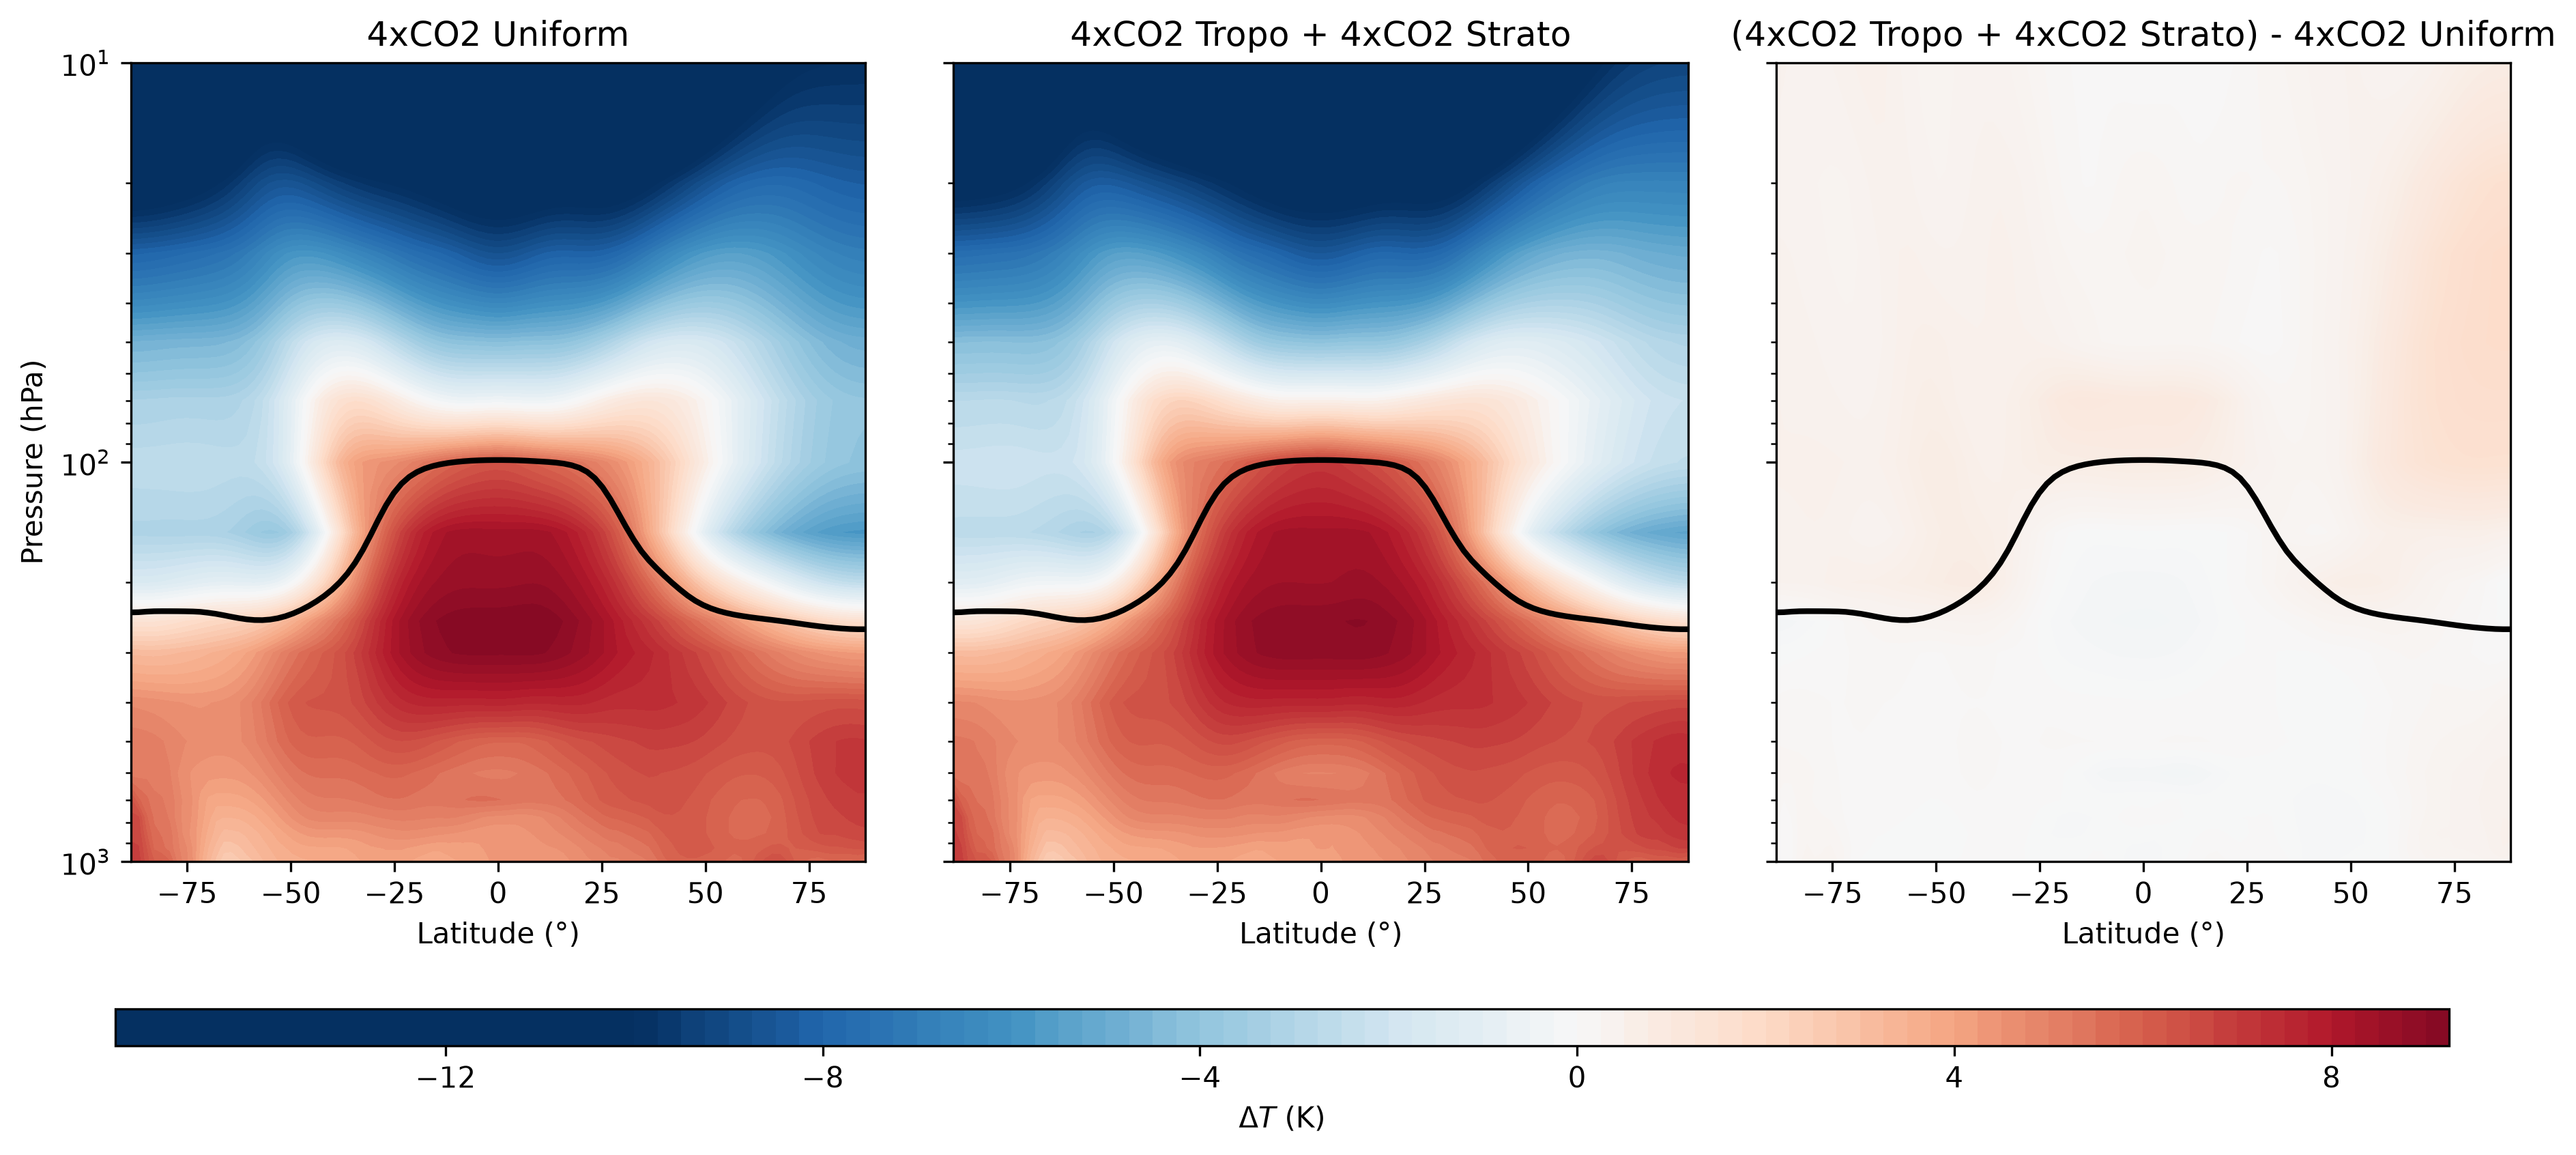
\includegraphics[width=\textwidth]{../../figures/initial_plots/t_uniform.png}
    \end{figure}
    \vfill
    \centering
    The temperature response of our forcings is \textbf{linear}.
\end{frame}
\section{Results}

\begin{frame}
    \frametitle{Temperature anomalies}
    \begin{figure}
        \centering
        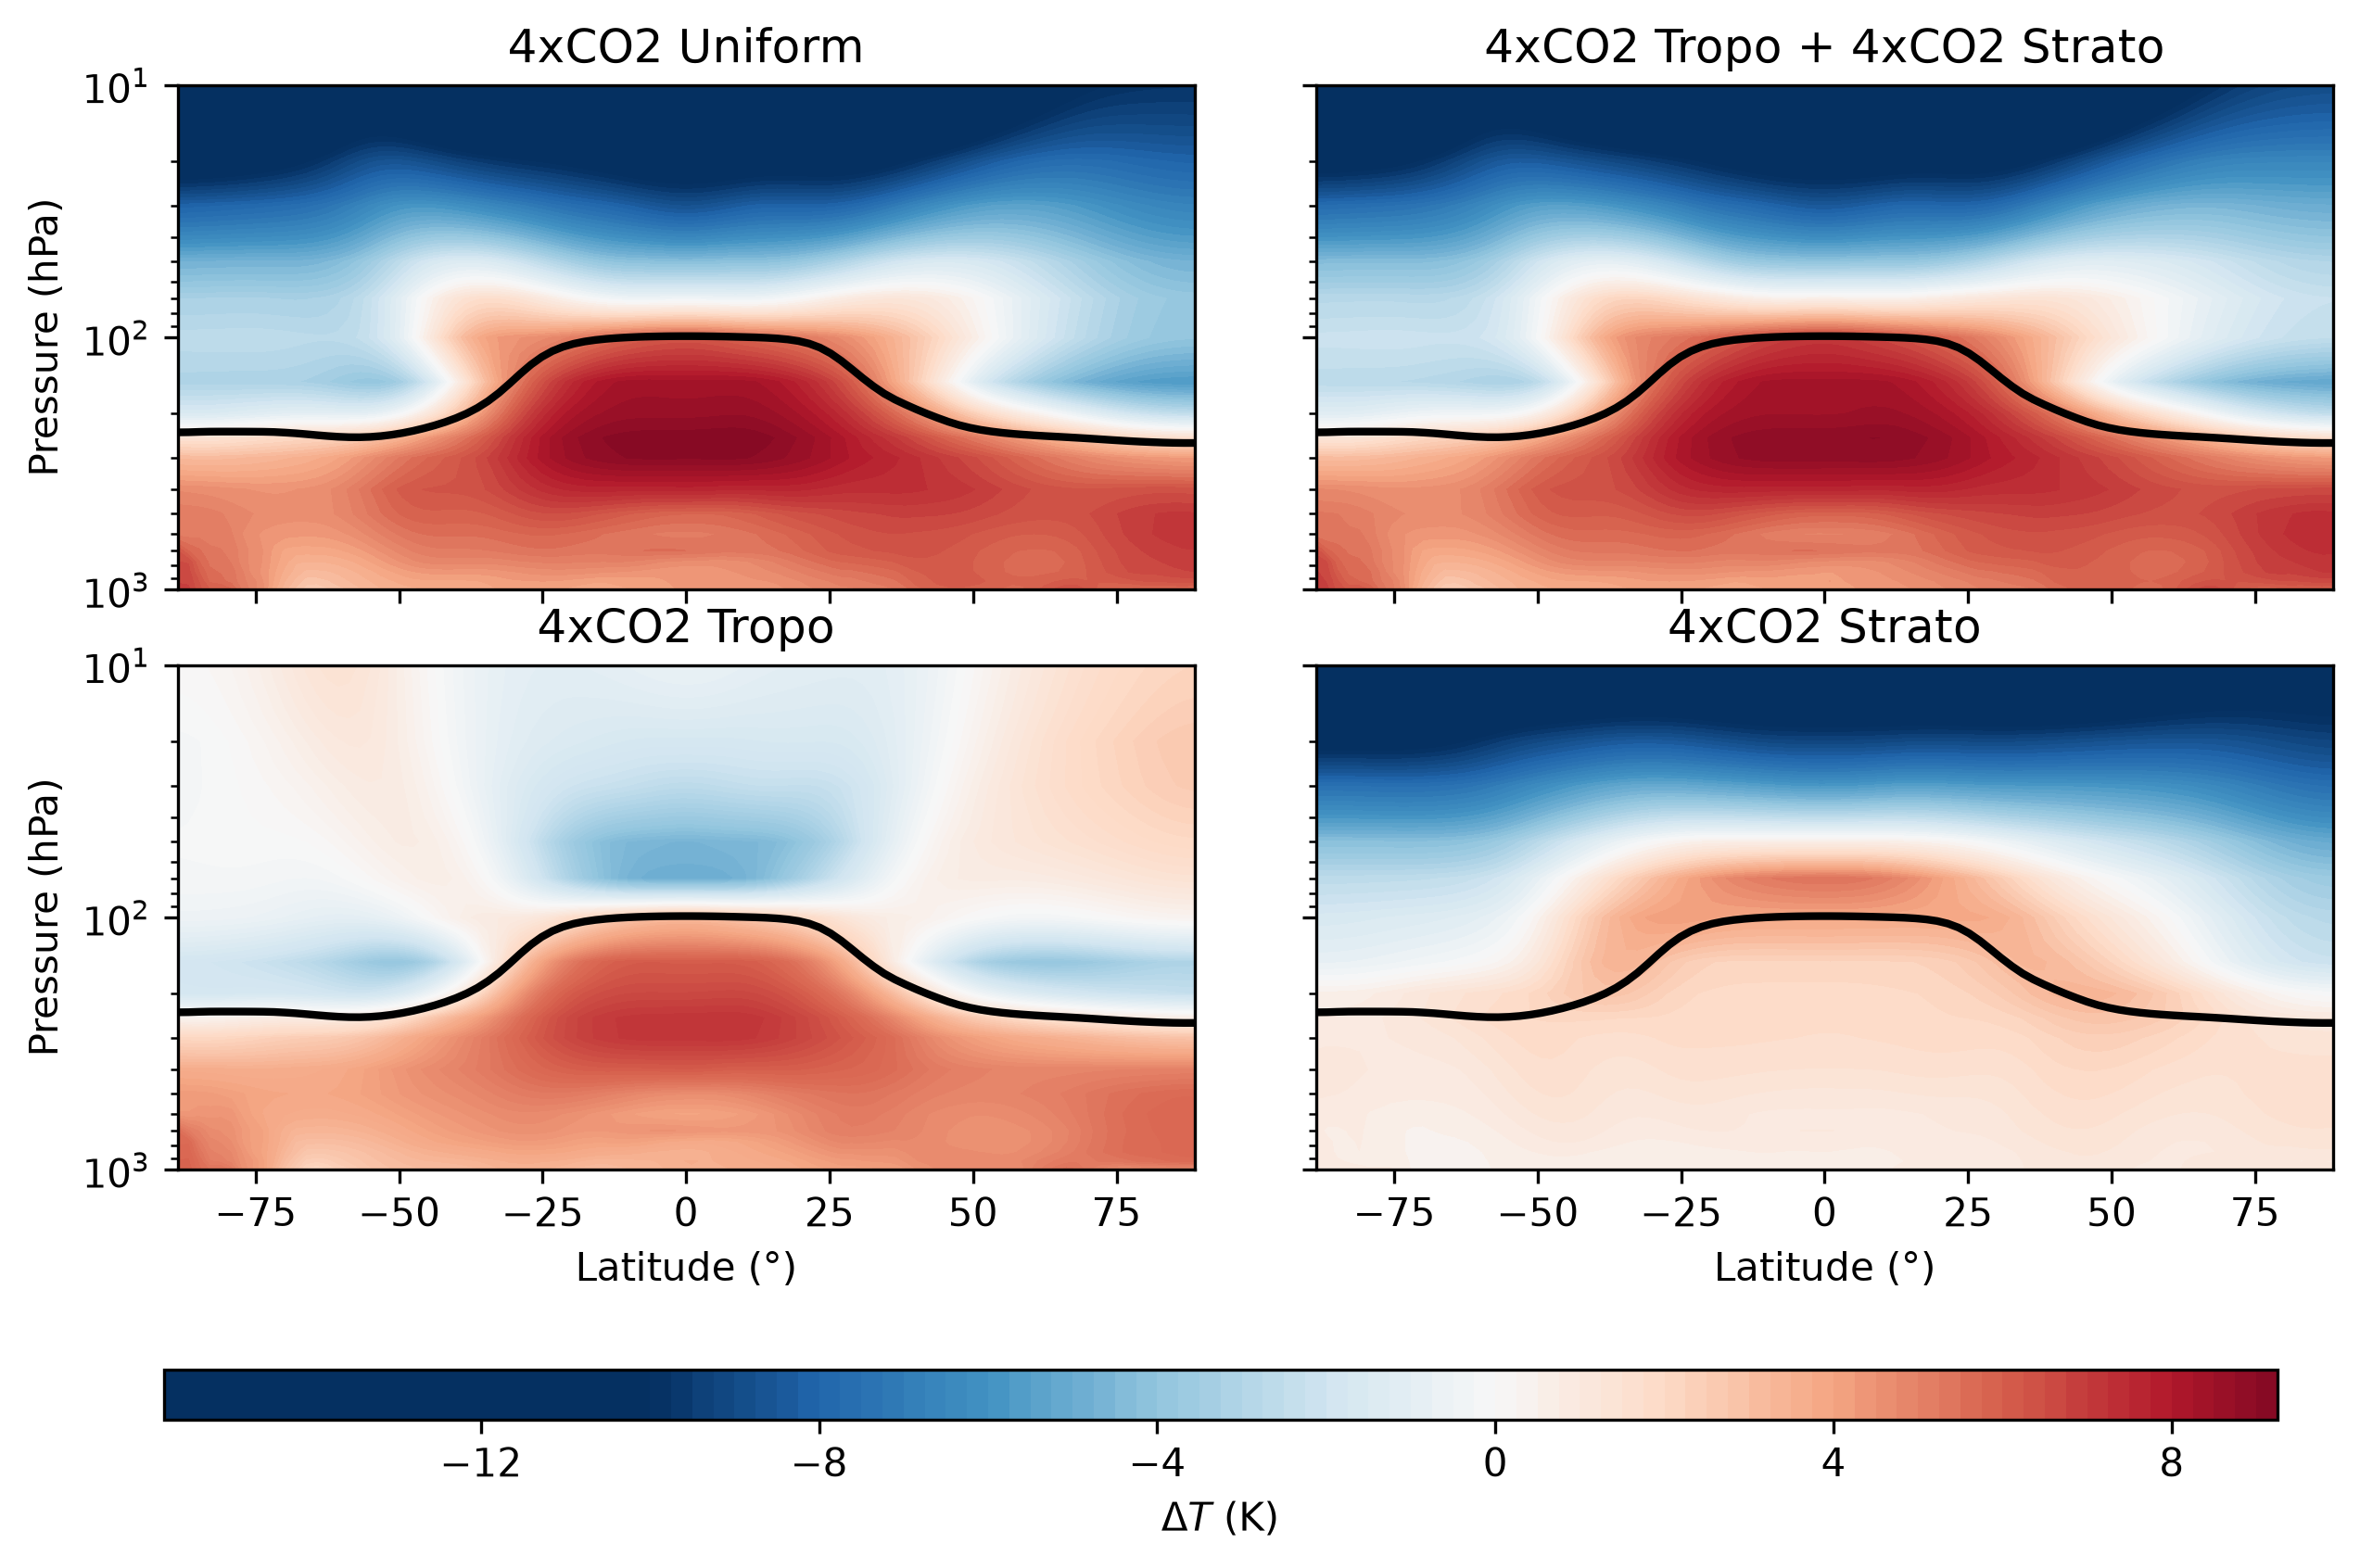
\includegraphics[width=0.7\textwidth]{../../figures/initial_plots/temperature.png}
    \end{figure}
    \begin{block}{}
        \begin{itemize}
            \item Tropospheric warming in 4xCO$_2$ Tropo
            \item Stratospheric cooling in 4xCO$_2$ Strato
        \end{itemize}
    \end{block}
\end{frame}

\begin{frame}
    \frametitle{RCE model}
    \begin{figure}
        \centering
        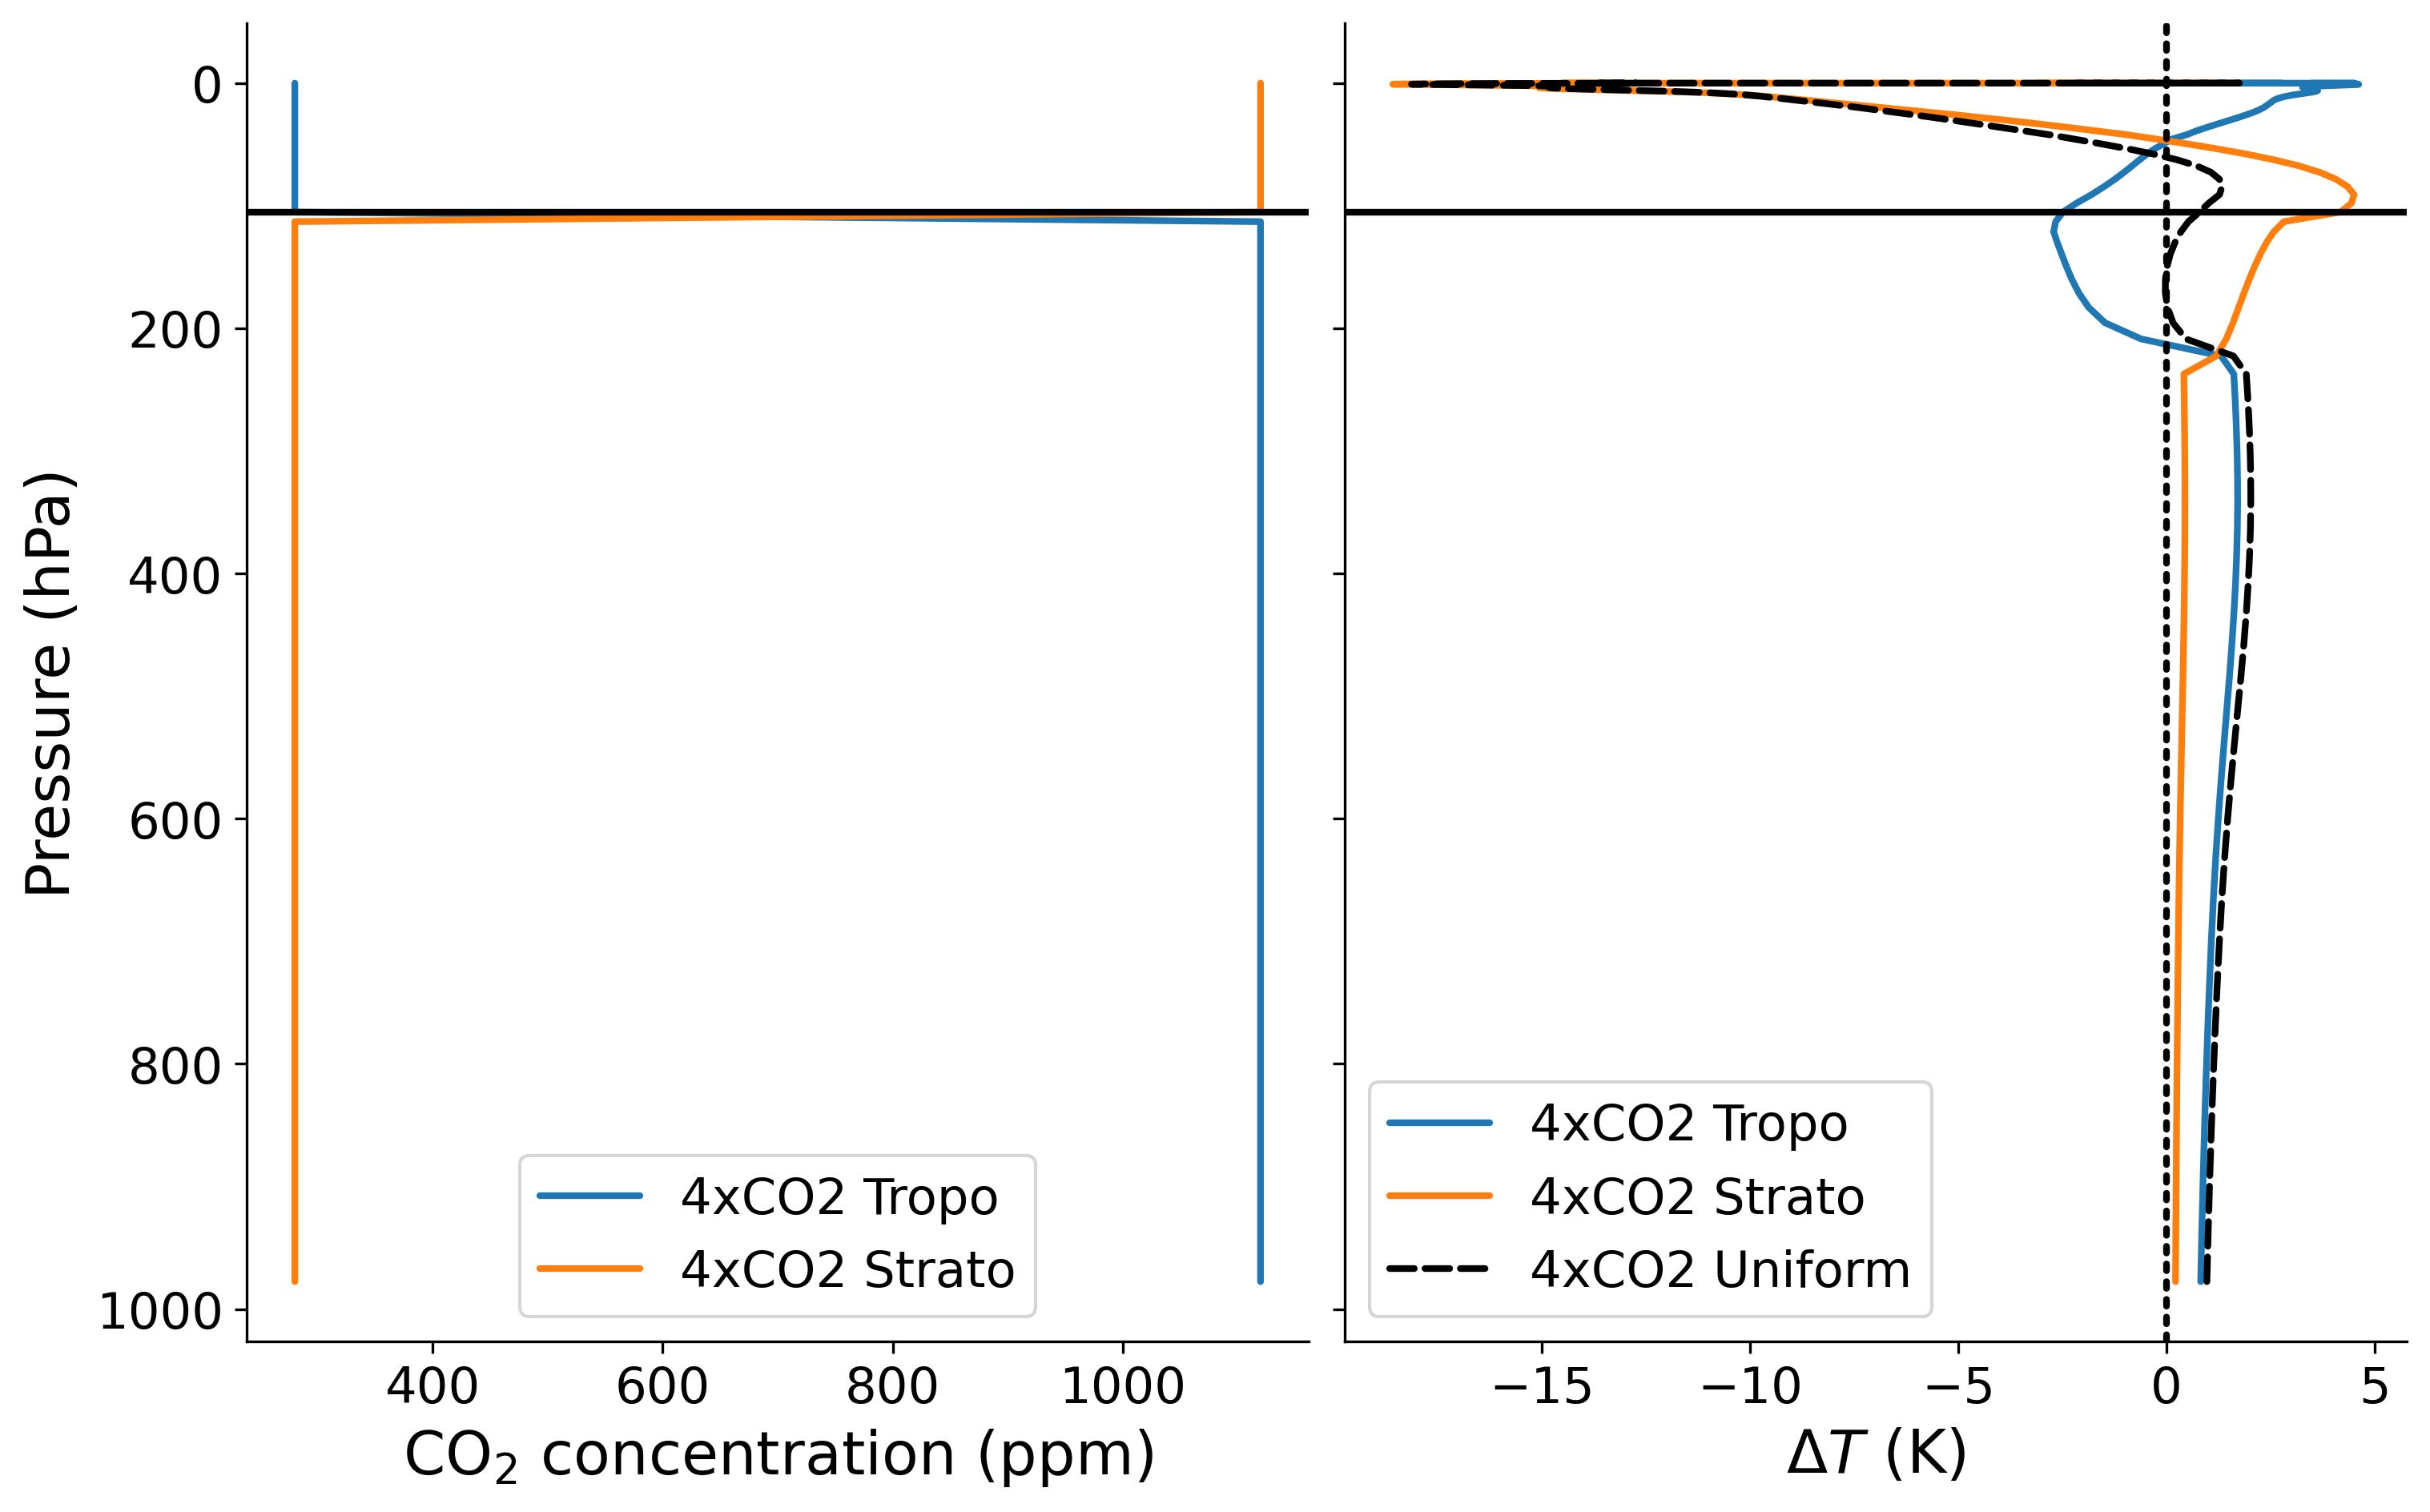
\includegraphics[width=0.8\textwidth]{../../figures/rce_simulations/konrad_slab_Tcold_CO2.png}
    \end{figure}
    \vfill
    \begin{center}
        Heating/cooling above the tropopause is due to changes in optical thickness
    \end{center}
\end{frame}

% \begin{frame}
%     \frametitle{Temperature anomalies}
%     \begin{figure}
%         \centering
%         
\includegraphics[width=0.6\textwidth]{figures/temperature.png}
%     \end{figure}
%     \begin{block}{Yet to be clarified}
%     \begin{itemize}
%         \item Stratospheric cooling in 4xCO$_2$ Tropo
%         \item Stratospheric warming in 4xCO$_2$ Strato
%         \item one-dimensional RCE model \textit{konrad}
%     \end{itemize}
%     \end{block}
% \end{frame}





\begin{frame}
    \frametitle{Zonally averaged circulation}
    \begin{figure}
        \centering
        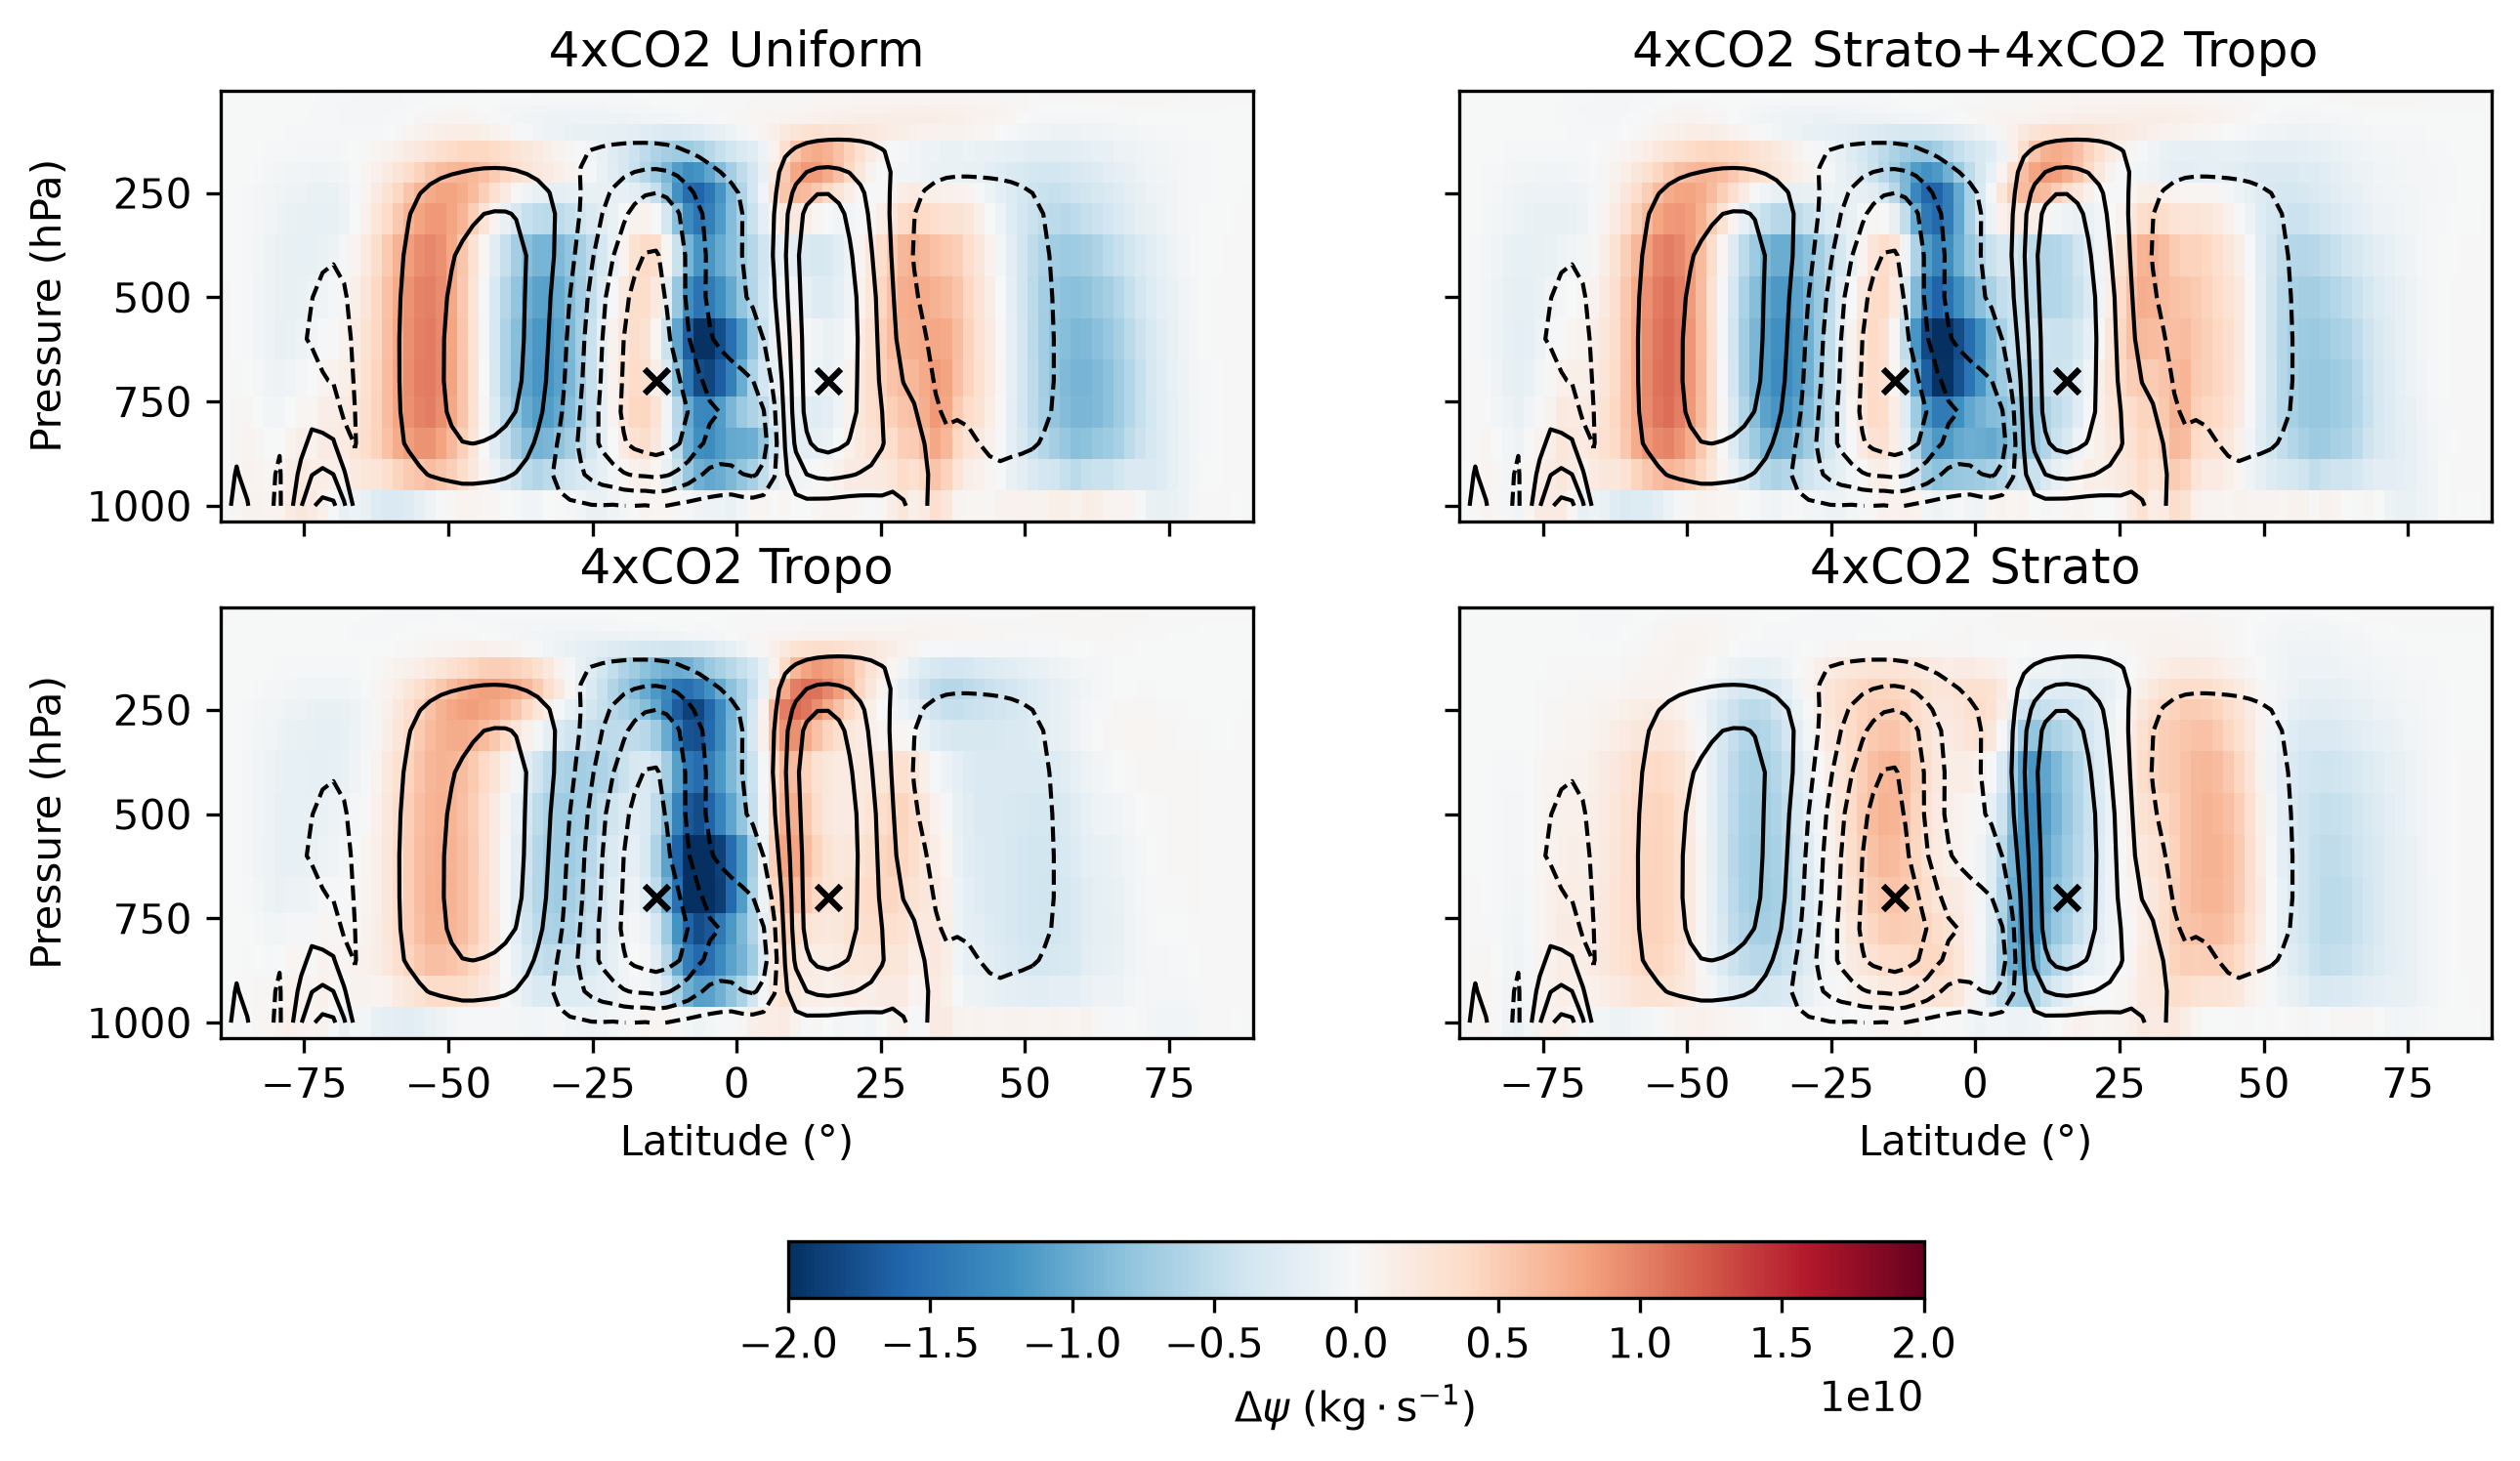
\includegraphics[width=\textwidth]{../../figures/initial_plots/streamfunc.png} %TODO
    \end{figure}
\end{frame}

\begin{frame}
  \frametitle{Changes in Hadley circulation}
\begin{table}[]
    \centering
    \begin{tabular}{c|ccc}
         &Uniform & Tropo & Strato \\ \toprule
        $\Delta\psi_\mathrm{max, NH}$& $-1.9\%$ & \textbf{$3.6\%$}& $-8.9\%$\\
        % $\Delta\psi_\mathrm{max, SH}$ & $-1.4\%$ & $5.6\%$ & $-5.7\%$\\ 
        $\Delta\Phi_\mathrm{H, NH}$  & $1.6\unit{\degree}$& $0.7\unit{\degree}$ &$0.7\unit{\degree}$
        % $\Delta\Phi_\mathrm{H, SH}$  & $-1.6\unit{\degree}$& $-1.0\unit{\degree}$ &$-0.6\unit{\degree}$\\
    \end{tabular}
    \label{tab:placeholder}
\end{table}
\begin{block}{Unexpected response}
    \begin{itemize}
        \item HC is \textbf{weakening} with stratospheric CO$_2$
        \item HC is \textbf{strengthening} with tropospheric CO$_2$
    \end{itemize}
\end{block}
\end{frame}

\begin{frame}
    %\frametitle{New question}
    \begin{alertblock}{New research question}
        Why is the HC weakening with stratospheric CO$_2$ forcing but strengthening with tropospheric CO$_2$ forcing?
    \end{alertblock}\pause
    \begin{block}{Methodology}
        Employ energy budget framework of the atmosphere to explain this behavior.
    \end{block}
\end{frame}


\section{Analysis}

\begin{frame}
    \frametitle{The energetic framework}
    \begin{figure}
        \centering
        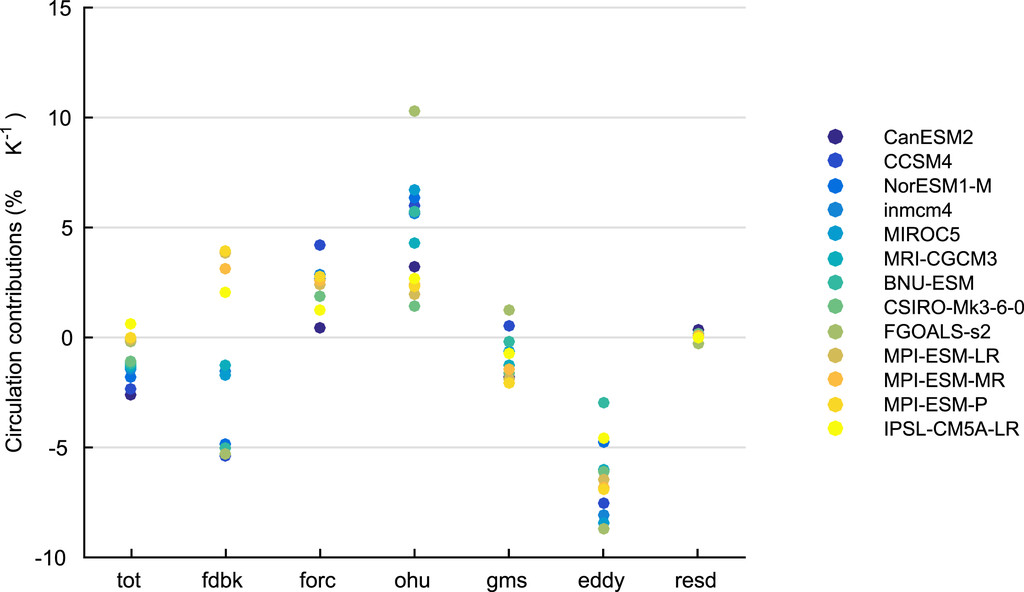
\includegraphics[width=0.85\textwidth]{../../figures/literature/Feldl_HC_decomposition.jpg}
        \caption{Contributions to changes in Hadley circulation for multiple models \parencite{feldlCharacterizingHadleyCirculation2016}.}
    \end{figure}
\end{frame}



\begin{frame}
    \frametitle{Energy transport}

    \begin{columns}
    \begin{column}{0.55\textwidth}
    \uncover<2->{
    \begin{block}{Flux to transport}  
        \begin{align*}
            R_\mathrm{TOA}&=\frac{\partial F}{\partial y}\\
            F_{ao}&=\int^\phi_{-\pi/2}\int^{2\pi}_0R_\mathrm{TOA}a^2\cos\phi\mathrm{d}\lambda\mathrm{d}\phi
        \end{align*}
    \end{block}}

    \end{column}
    \begin{column}{0.45\textwidth}
        \begin{figure}
            \centering
            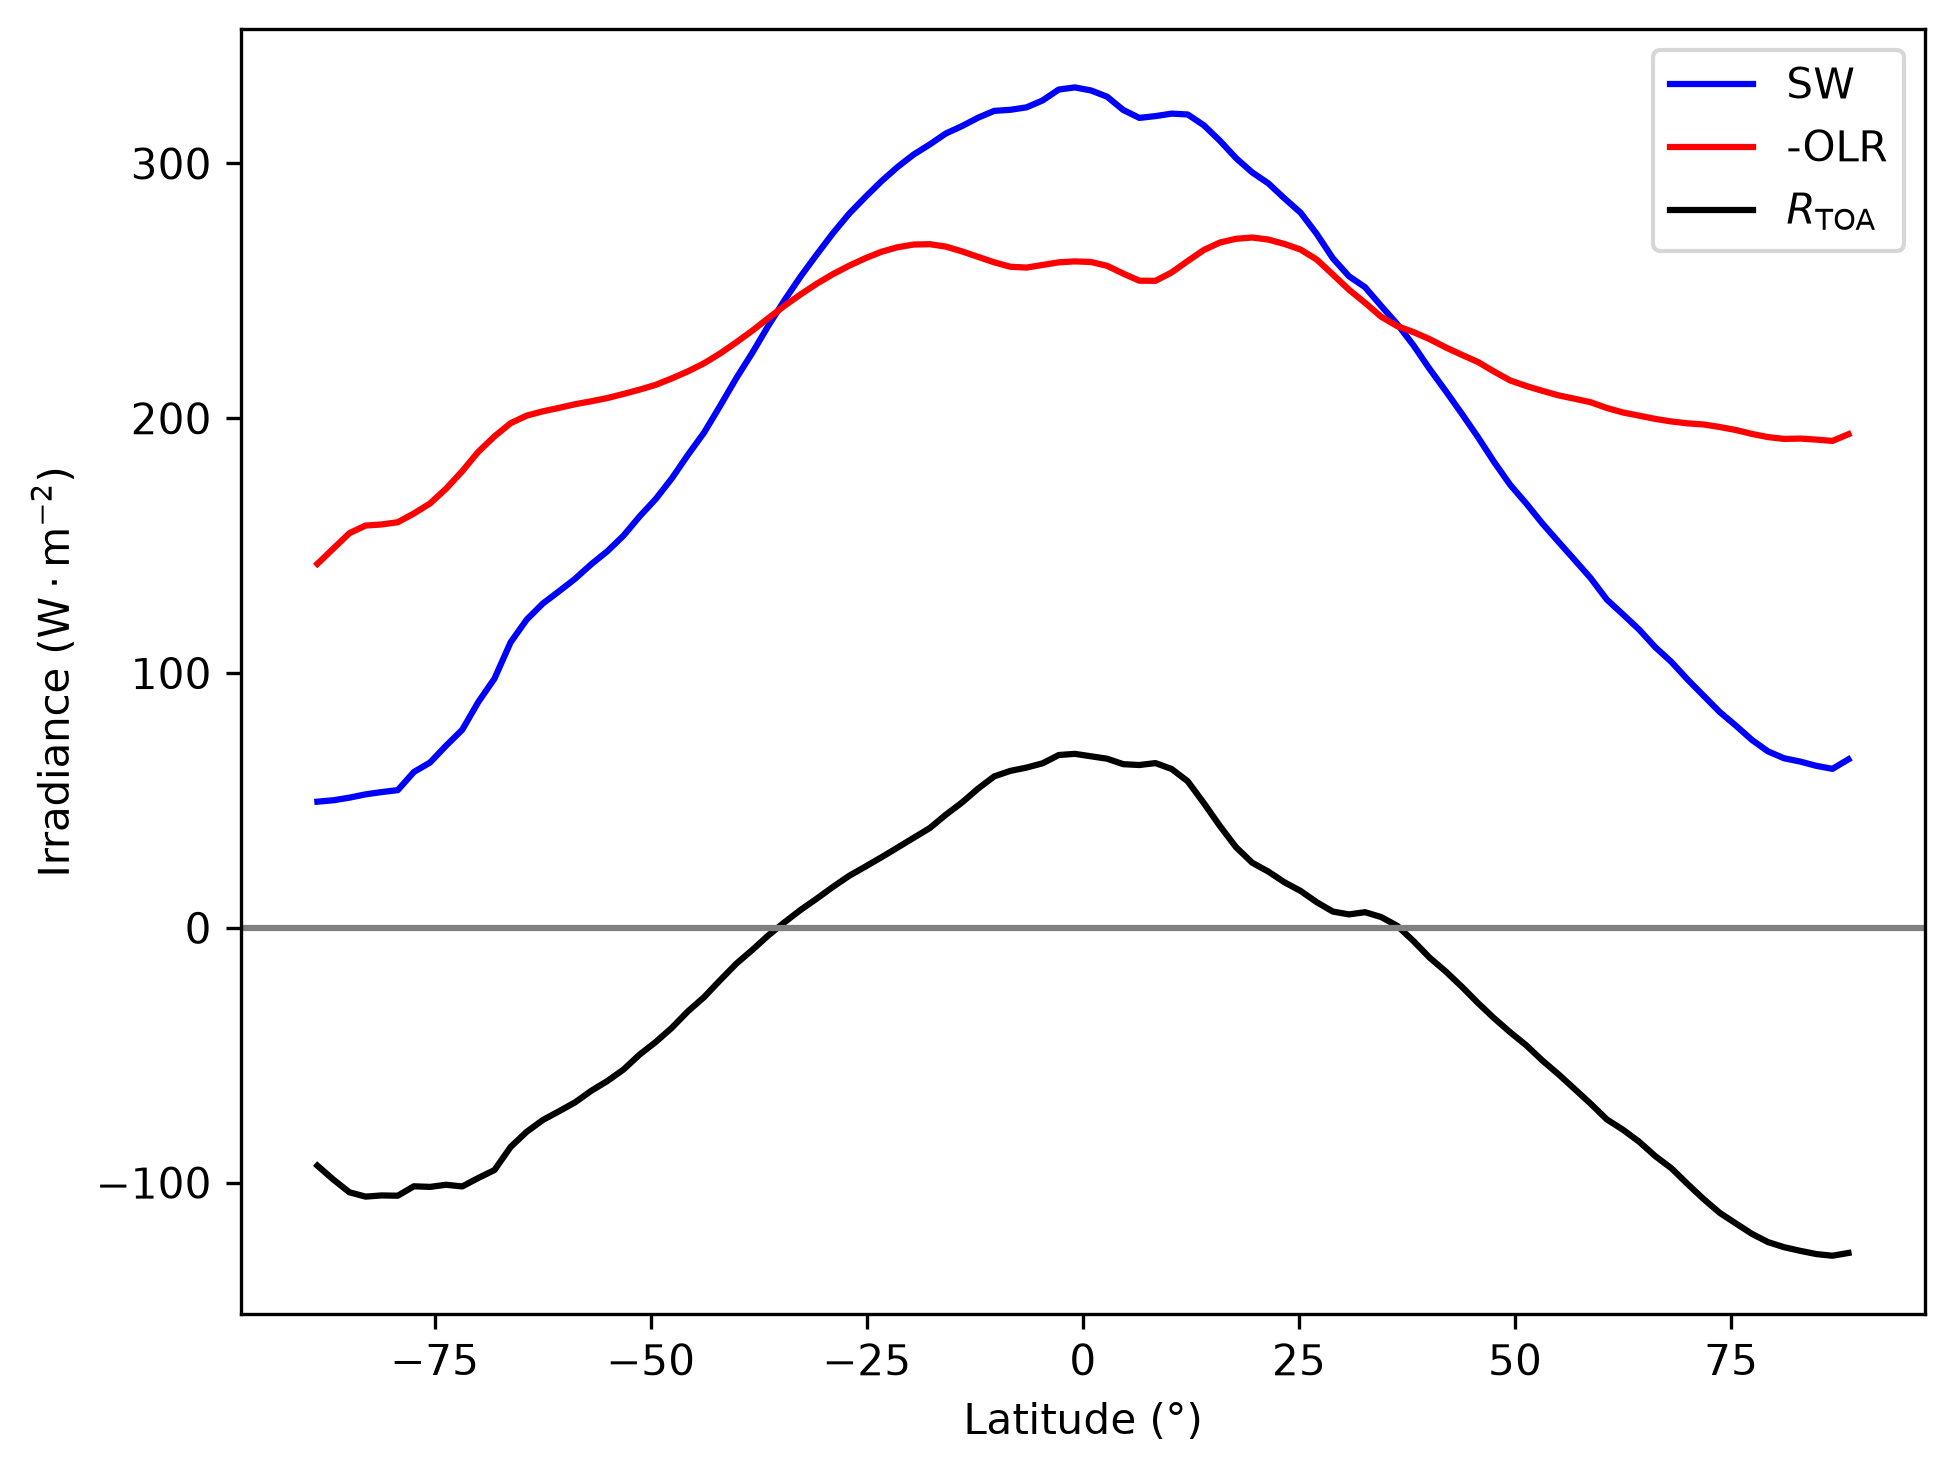
\includegraphics[width=\textwidth]{../../figures/initial_plots/irradiance.png}
        \end{figure}
    \end{column}
    \end{columns}
\end{frame}

\begin{frame}
    \frametitle{Energy transport by the Hadley cell?}

    \begin{columns}
    \begin{column}{0.45\textwidth}  %%<--- here
    \begin{block}{Linearisation}  
        \begin{align*}
            F_\mathrm{HC}&=\psi_\mathrm{max}H \\
            H&\sim\frac{1}{\psi_\mathrm{max}}\int^{p_s}_0[\Bar{v}][\Bar{h}]\mathrm{d}p\\
            \frac{\delta\psi_\mathrm{max}}{\psi_\mathrm{max}}&=\frac{\delta F_\mathrm{HC}}{F_\mathrm{HC}}-\frac{\delta H}{H}
        \end{align*}
    \end{block}

    \end{column} \pause
    \begin{column}{0.55\textwidth}
        \begin{figure}
            \centering
            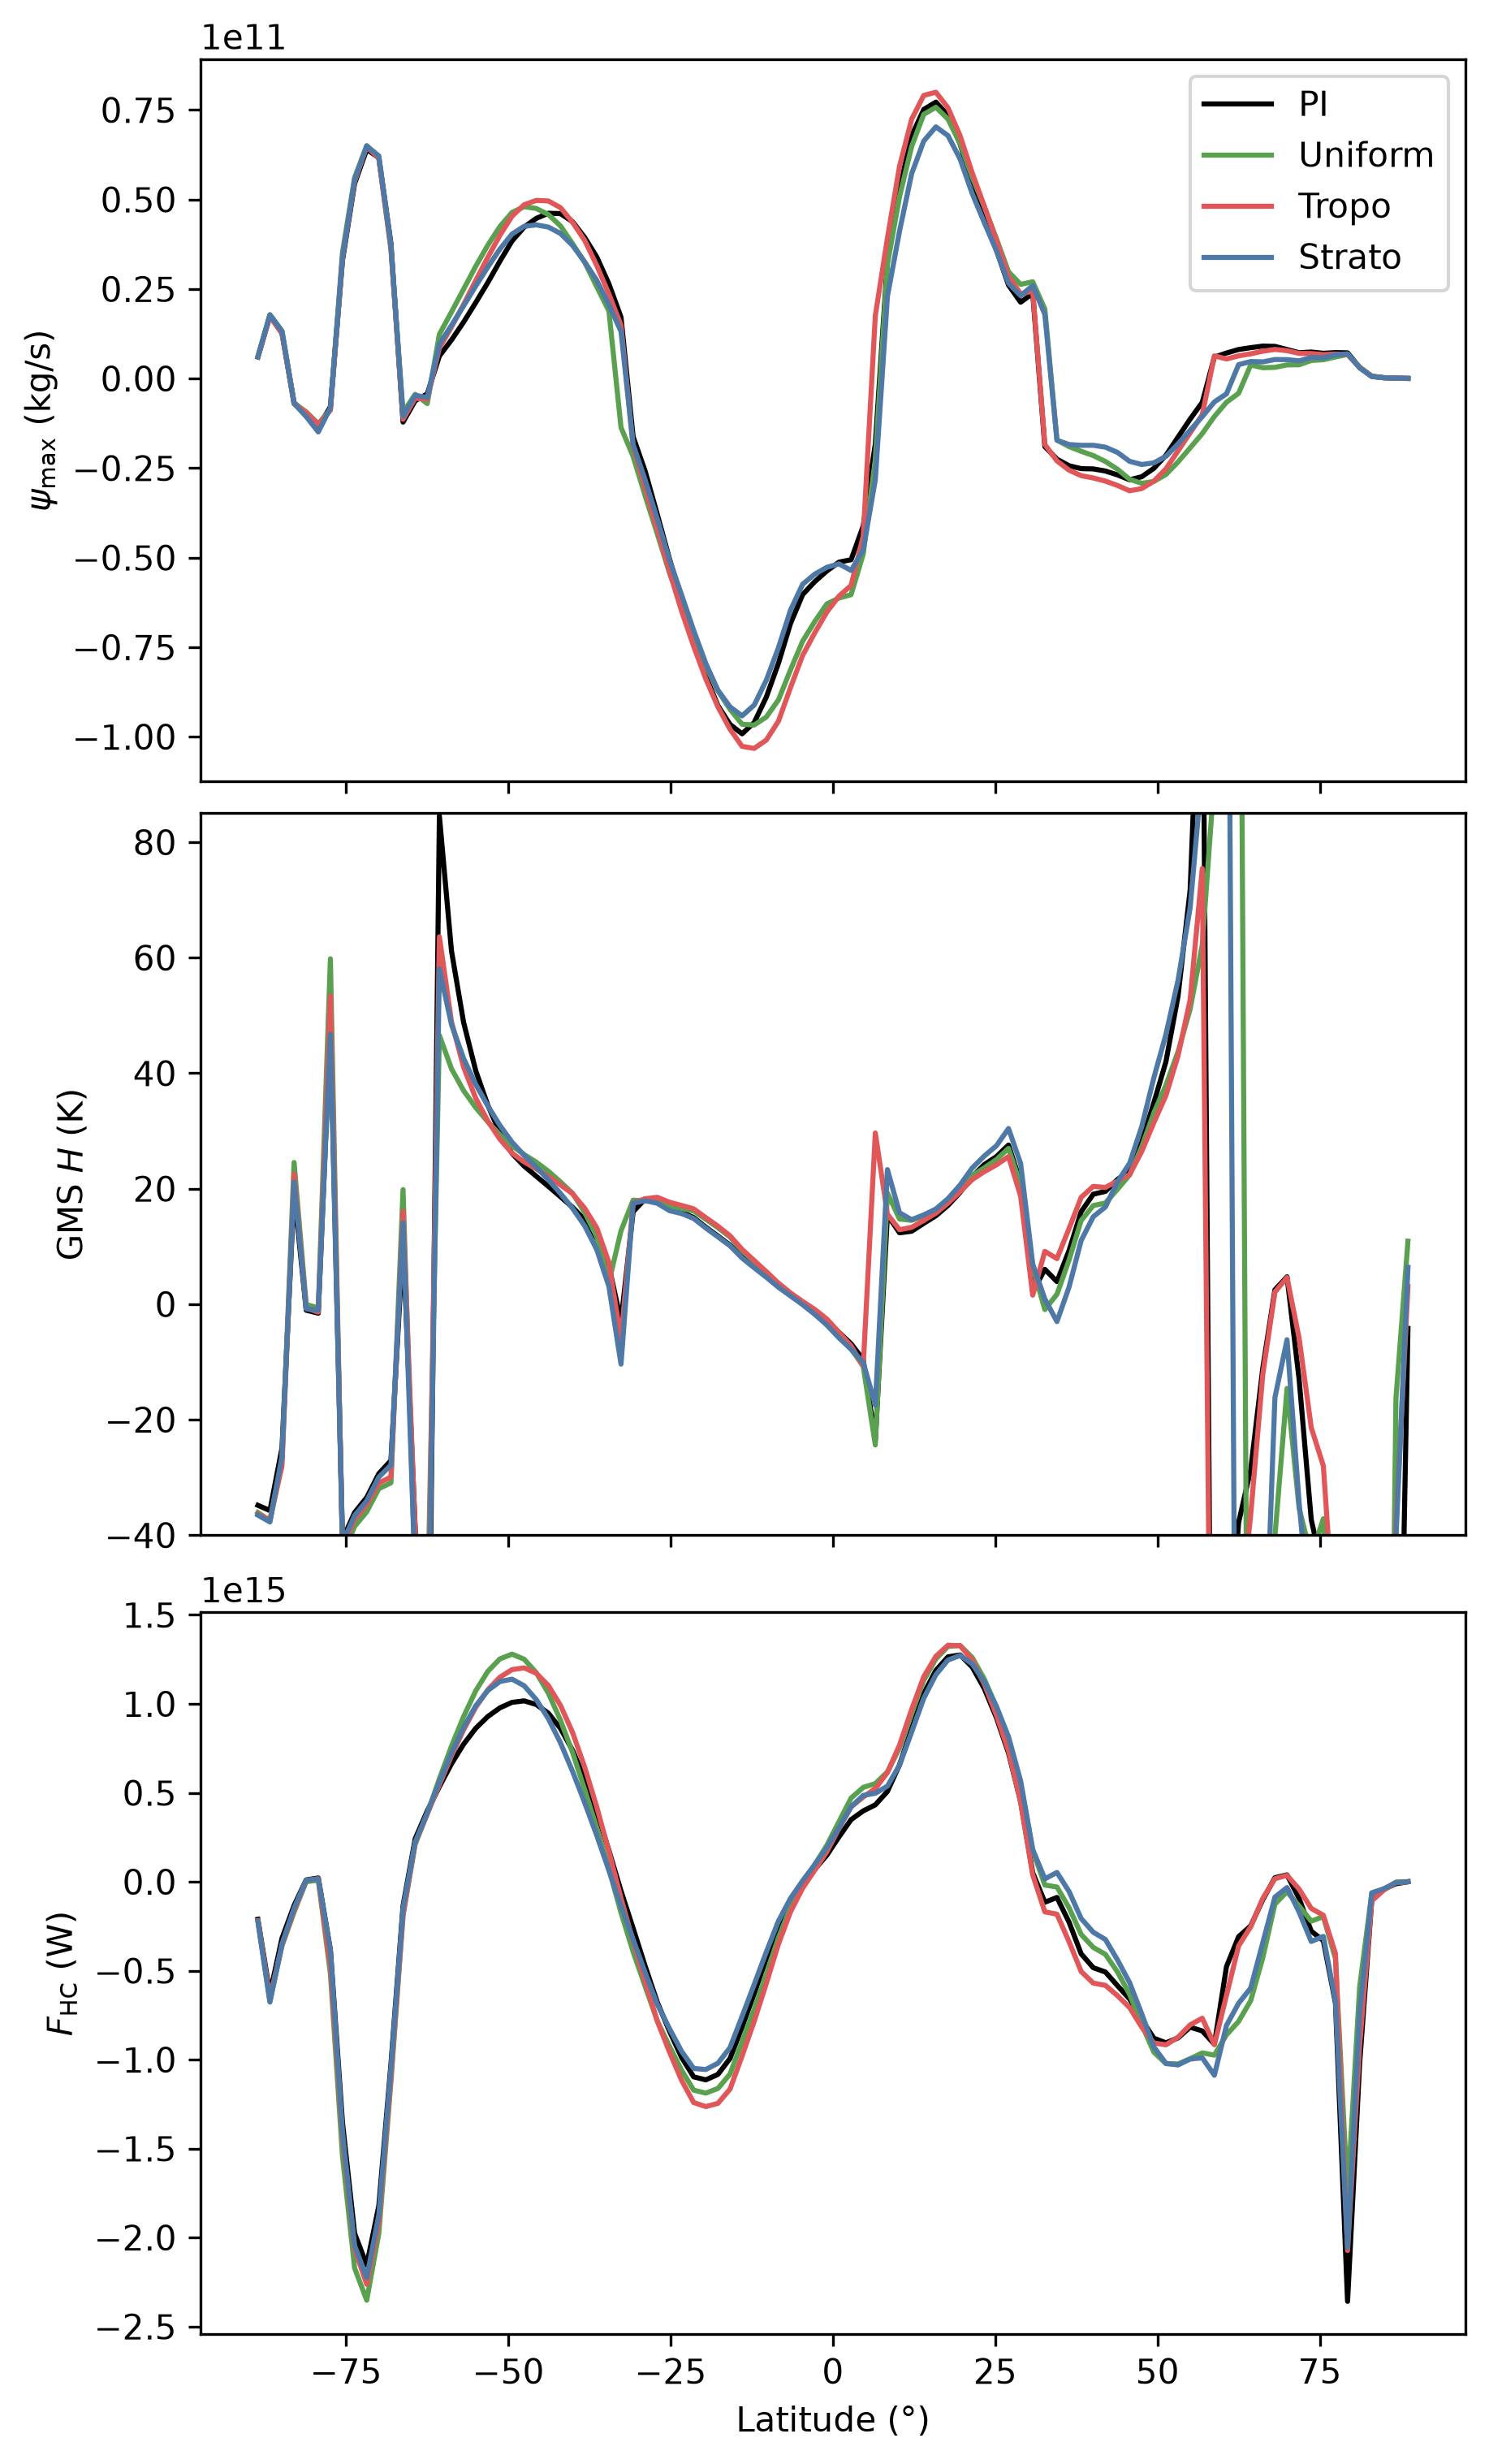
\includegraphics[height=0.8\textheight]{../../figures/energetic_framework/GMS_F_HC.png}
        \end{figure}
    \end{column}
    \end{columns}
\end{frame}

\begin{frame}
    \frametitle{GMS weakens the circulation}
    \begin{figure}
        \centering
        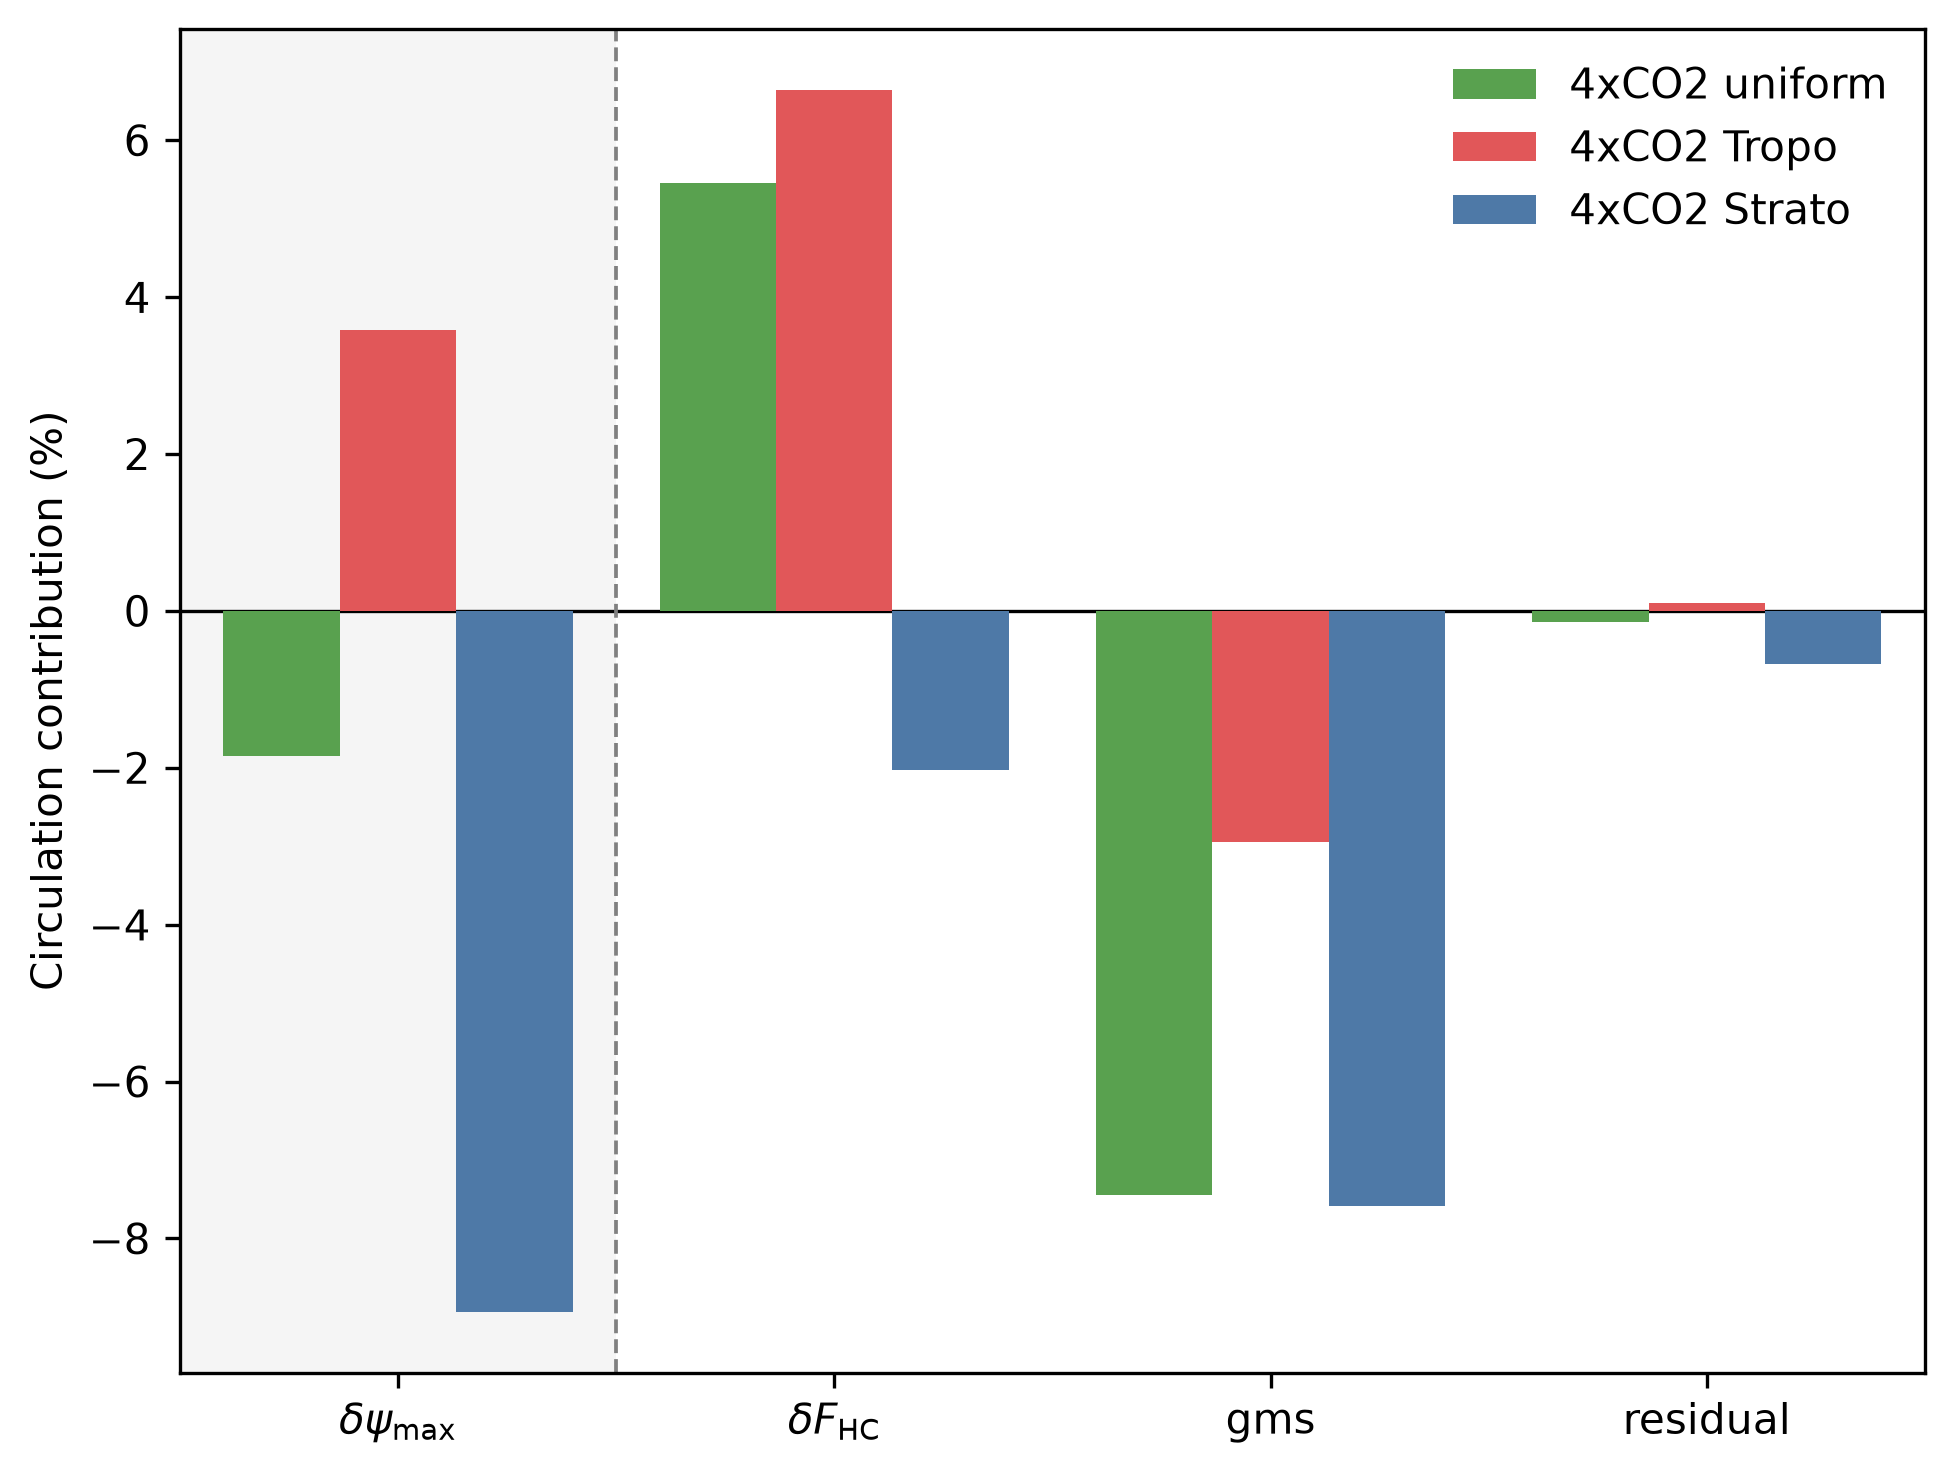
\includegraphics[width=0.8\textwidth]{../../figures/energetic_framework/contributions_simple.png}
    \end{figure}
\end{frame}


\begin{frame}
    \frametitle{Eddy energy transport}

    \begin{columns}
    \begin{column}{0.45\textwidth}  %%<--- here
    \begin{block}{Linearisation}  
        \begin{align*}
            F_\mathrm{HC}&=F_\mathrm{a}-F_\mathrm{e}\\
            \frac{\delta\psi_\mathrm{max}}{\psi_\mathrm{max}}&=\frac{\delta F_\mathrm{a}}{F_\mathrm{HC}}-\frac{\delta F_\mathrm{e}}{F_\mathrm{HC}}-\frac{\delta H}{H}
        \end{align*}
    \end{block}

    \end{column}
    \begin{column}{0.55\textwidth}
        \begin{figure}
            \centering
            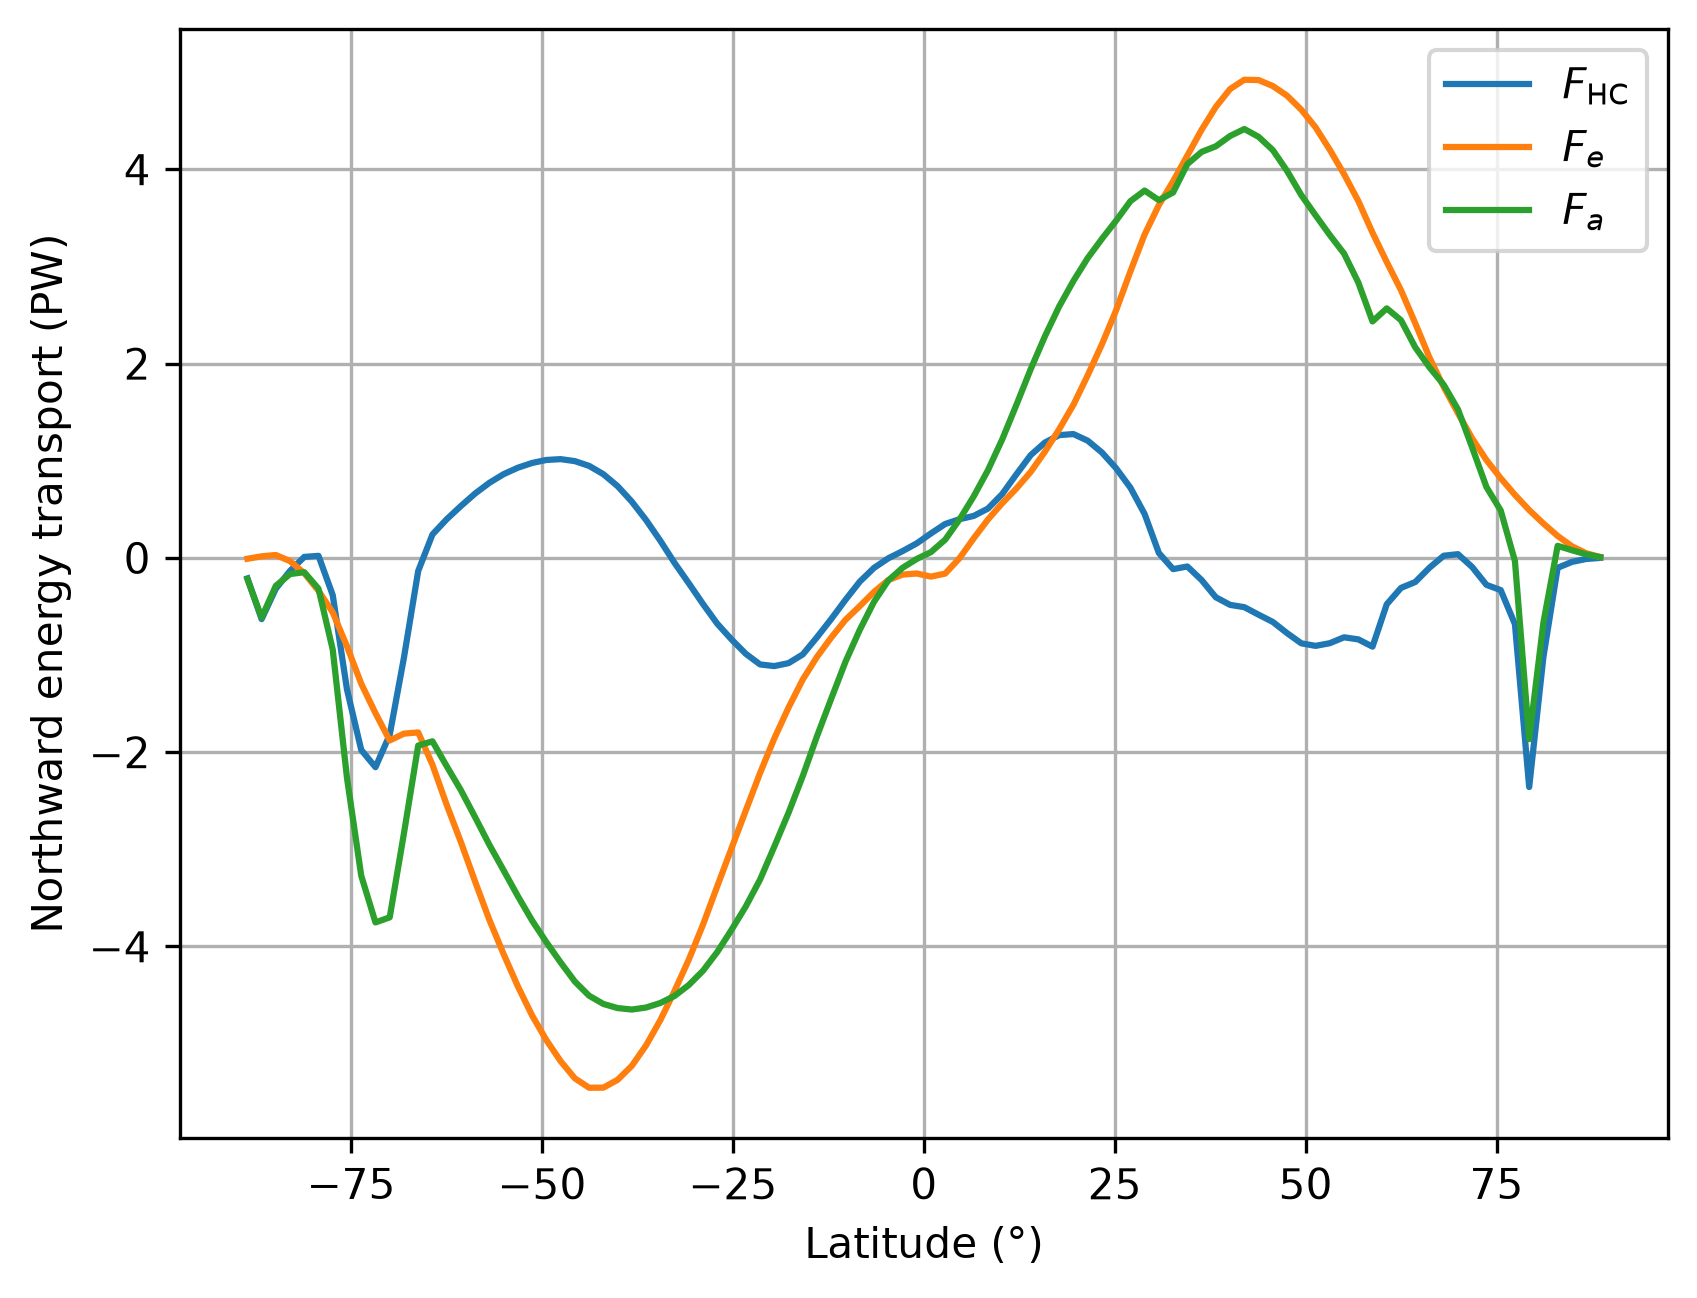
\includegraphics[width=\textwidth]{../../figures/energetic_framework/transport_decomposition_HC_eddies.png}
        \end{figure}
    \end{column}
    \end{columns}
\end{frame}

\begin{frame}
    \frametitle{Oppsing eddy contributions}
    \begin{figure}
        \centering
        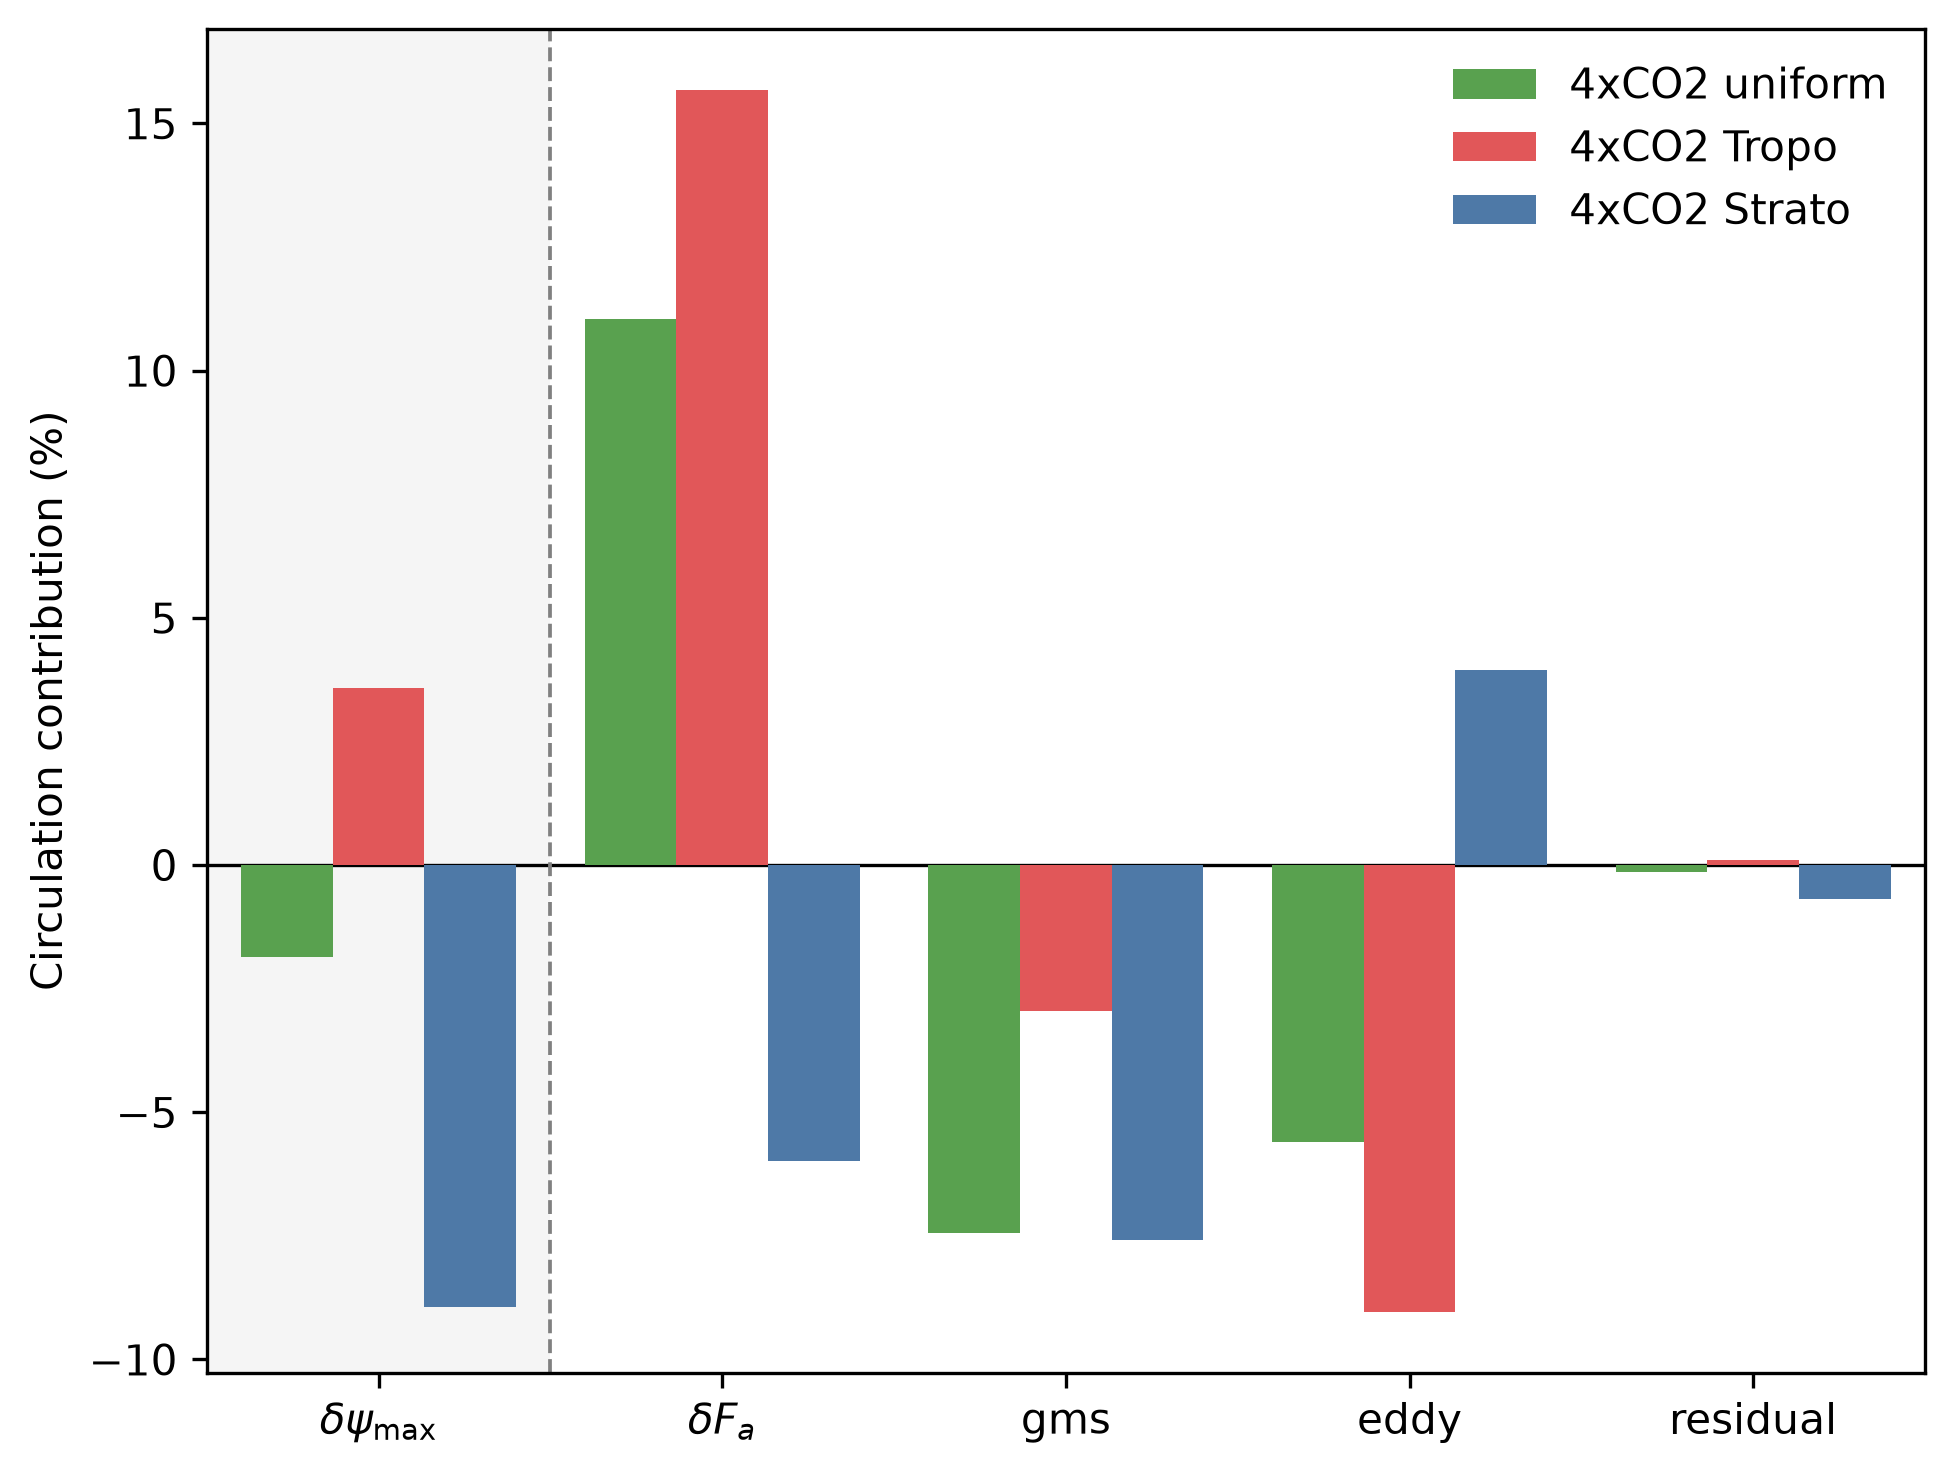
\includegraphics[width=0.8\textwidth]{../../figures/energetic_framework/contributions_eddies_NH.png}
    \end{figure}
\end{frame}
\begin{frame}
    \frametitle{Meridional temperature gradient and jet strength}
    \begin{figure}
        \centering
        
\includegraphics[width=\textwidth]{eddy_flux/temperature_jet_stream.png}
    \end{figure}
\end{frame}
\begin{frame}
    \frametitle{Forcing and feedbacks}

    \begin{columns}
    \begin{column}{0.55\textwidth}  %%<--- here
    \begin{block}{Linearisation}  
        \begin{align*}
            \Delta R_\mathrm{TOA}&=\sum_i\lambda_i\Delta T_s+R_f\\
            \frac{\delta\psi_\mathrm{max}}{\psi_\mathrm{max}}&=\frac{\delta F_\mathrm{forc}}{F_\mathrm{HC}}+\frac{\delta F_\mathrm{fdb}}{F_\mathrm{HC}}-\frac{\delta F_\mathrm{e}}{F_\mathrm{HC}}-\frac{\delta H}{H}
        \end{align*}
    \end{block}

    \end{column}\pause
    \begin{column}{0.45\textwidth}
        \begin{figure}
            \centering
            
\includegraphics[width=0.9\textwidth]{energetic_framework/forcing_fixed_SST_scale_fill.png}
        \end{figure}
    \end{column}
    \end{columns}
\end{frame}

\begin{frame}
    \frametitle{Forcing contributions}
    \begin{figure}
        \centering
        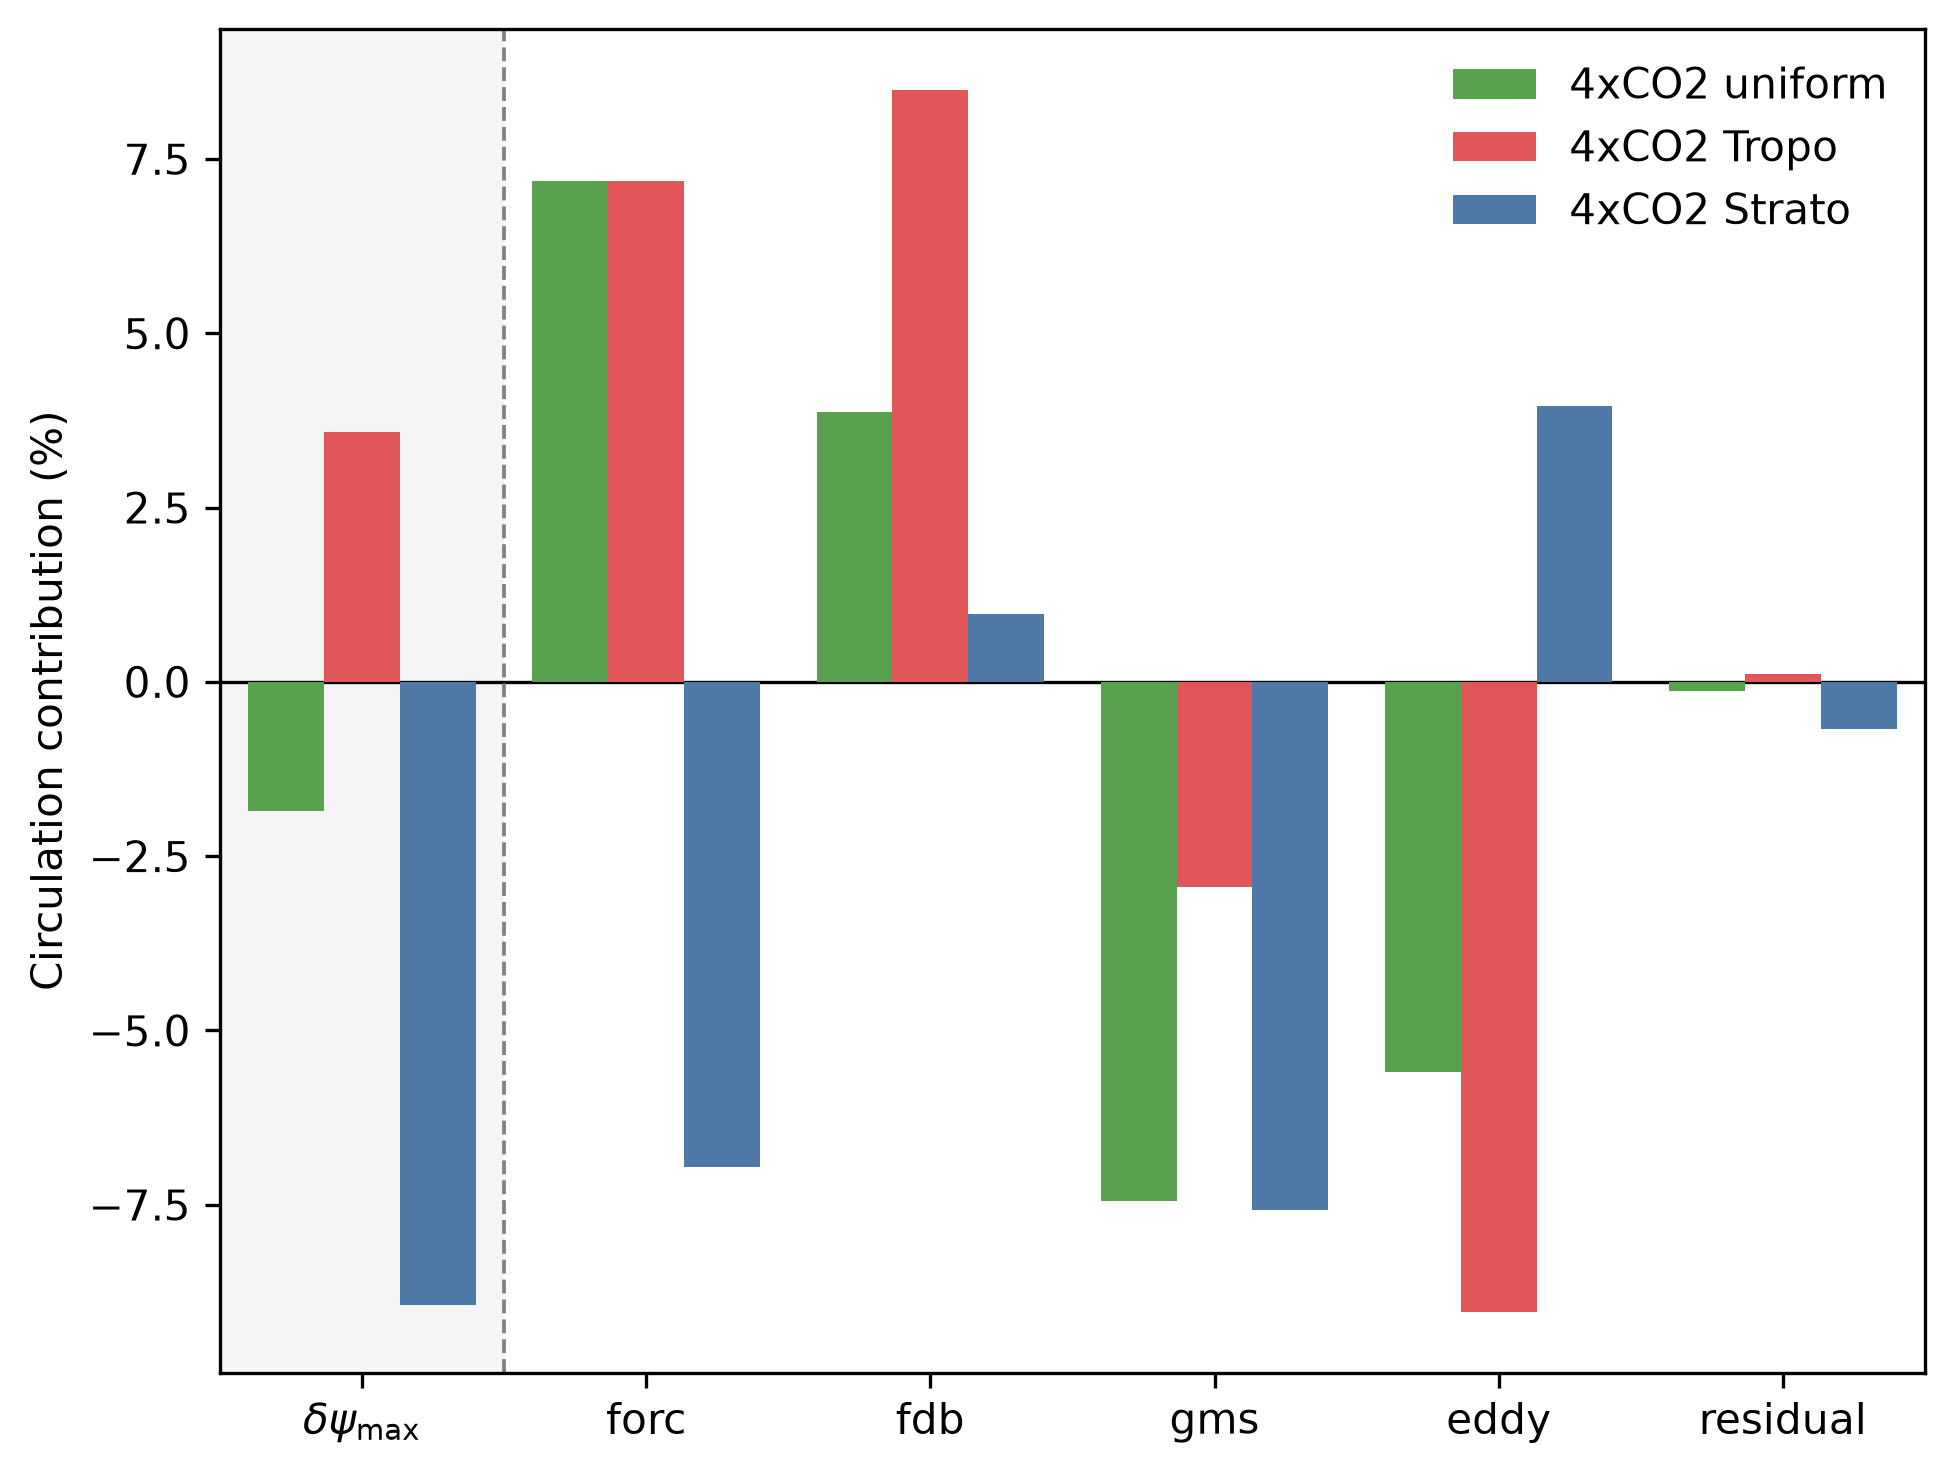
\includegraphics[width=0.8\textwidth]{../../figures/energetic_framework/contributions_eddy_forcing_NH.png}
    \end{figure}
\end{frame}
\begin{frame}
    \frametitle{Meridional forcing structure}
        \begin{figure}
            \centering
            
\includegraphics[width=0.8\textwidth]{energetic_framework/forcing_fixed_SST_scale_fill.png}
        \end{figure}
\end{frame}
\begin{frame}
    \frametitle{Summary}
    \begin{alertblock}{Research question}
        How does the atmosphere respond to forcing in the troposphere compared to the stratosphere?
    \end{alertblock} \pause
    \begin{block}{Key takeaways}
        \begin{itemize}[<+->]
            \item<2-> Tropospheric and stratospheric CO$_2$ contribute very differently to Hadley circulation changes.
            \item<3-> HC is strengthening with 4xCO$_2$ in the troposphere and weakening with with 4xCO$_2$ in the stratosphere. 
            \item<4->Circulation changes can be attributed to changes in forcing, feedback, GMS, and eddies.
            \item<5-> Meridional forcing structure as the main driver for the different circulation response.
        \end{itemize}
    \end{block}
    \pause
    \vfill 
    \pause
    \begin{center}
    \pause
    \pause
    \textbf{Thank you for your attention!}
    \end{center} 
\end{frame}



%% Prevent urls running into margins in bibliography
\setcounter{biburlnumpenalty}{7000}
\setcounter{biburllcpenalty}{7000}
\setcounter{biburlucpenalty}{7000}

\begin{frame}[allowframebreaks]
    \frametitle{References}
    %%  Add the bibliography
    \printbibliography[]
\end{frame}

\backupbegin

\begin{frame}
    \frametitle{}
    \begin{figure}
        \centering
        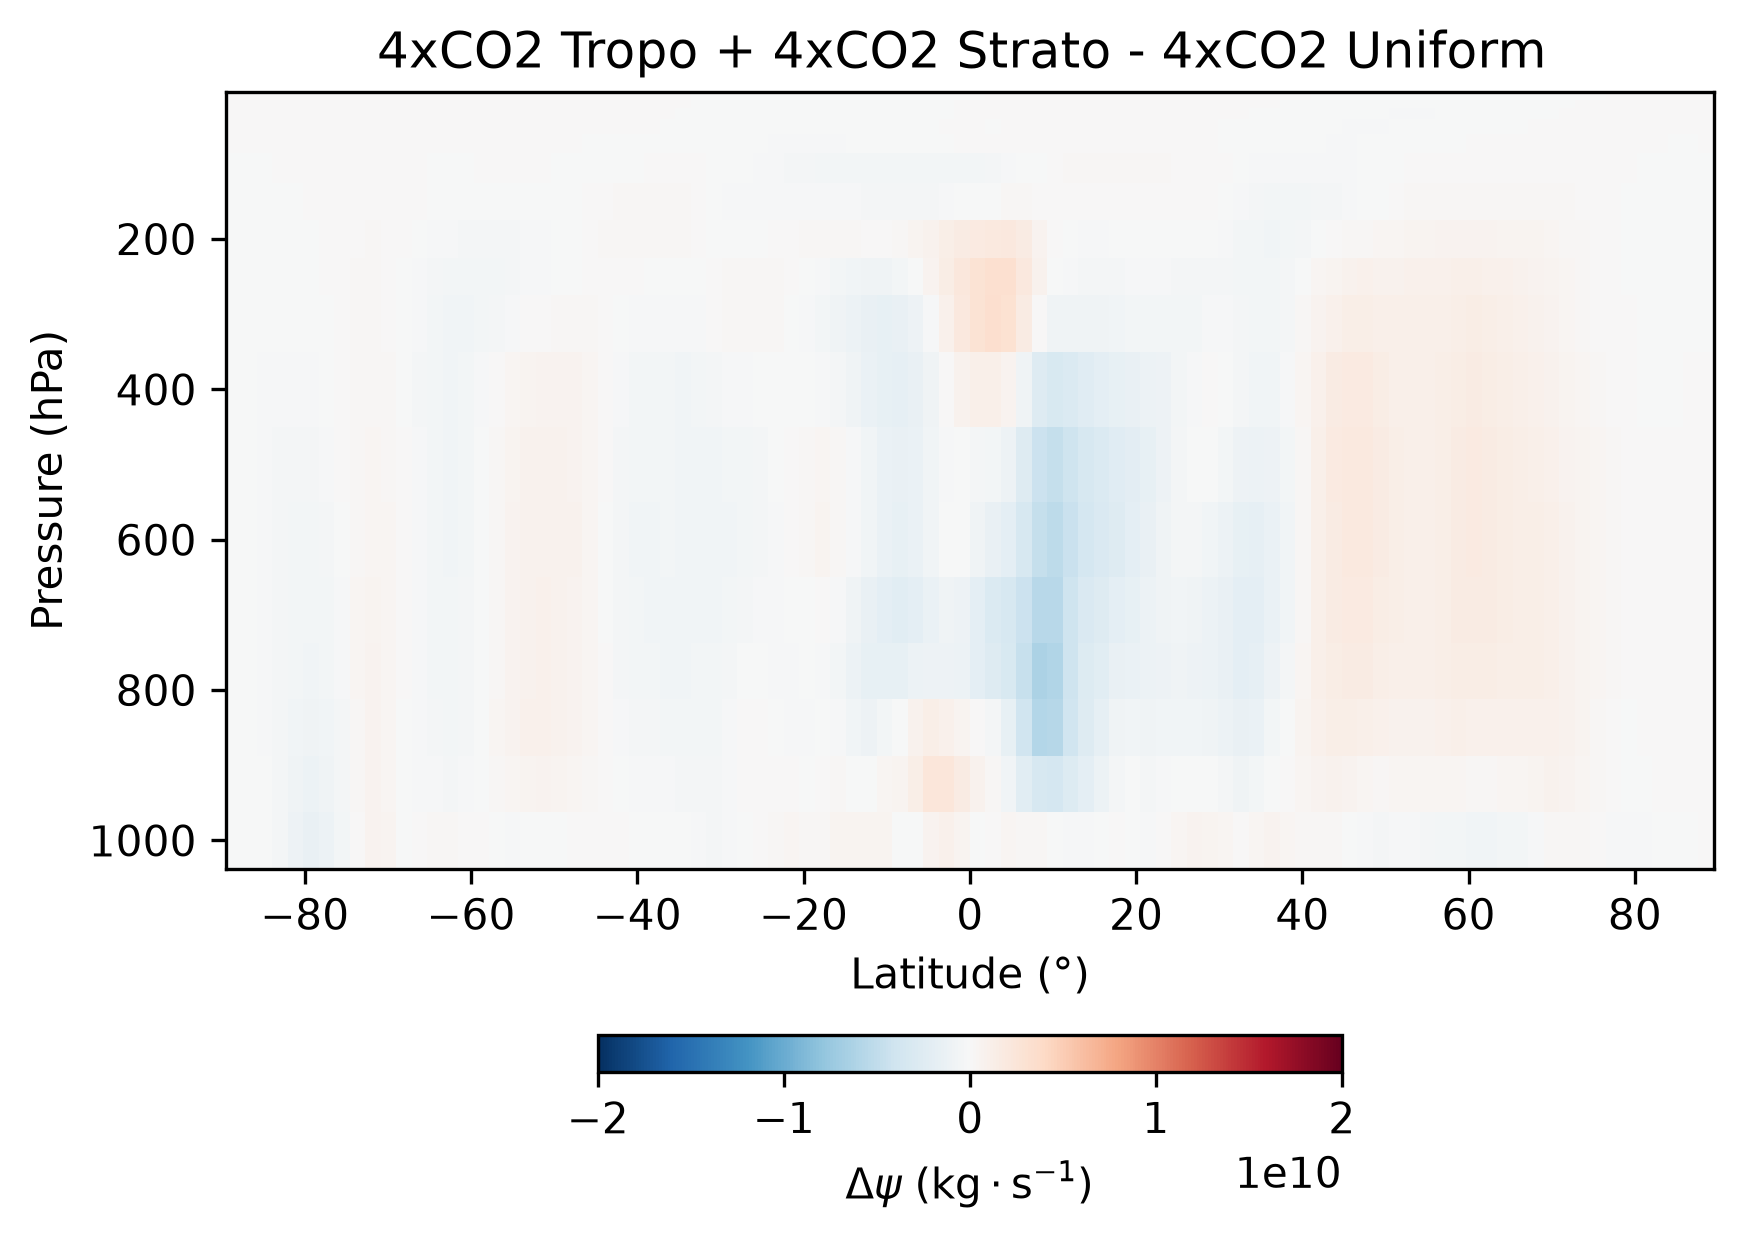
\includegraphics[width=\textwidth]{../../figures/initial_plots/difference_stream_function.png}
    \end{figure}
\end{frame}

\begin{frame}
    \frametitle{}
    \begin{figure}
        \centering
        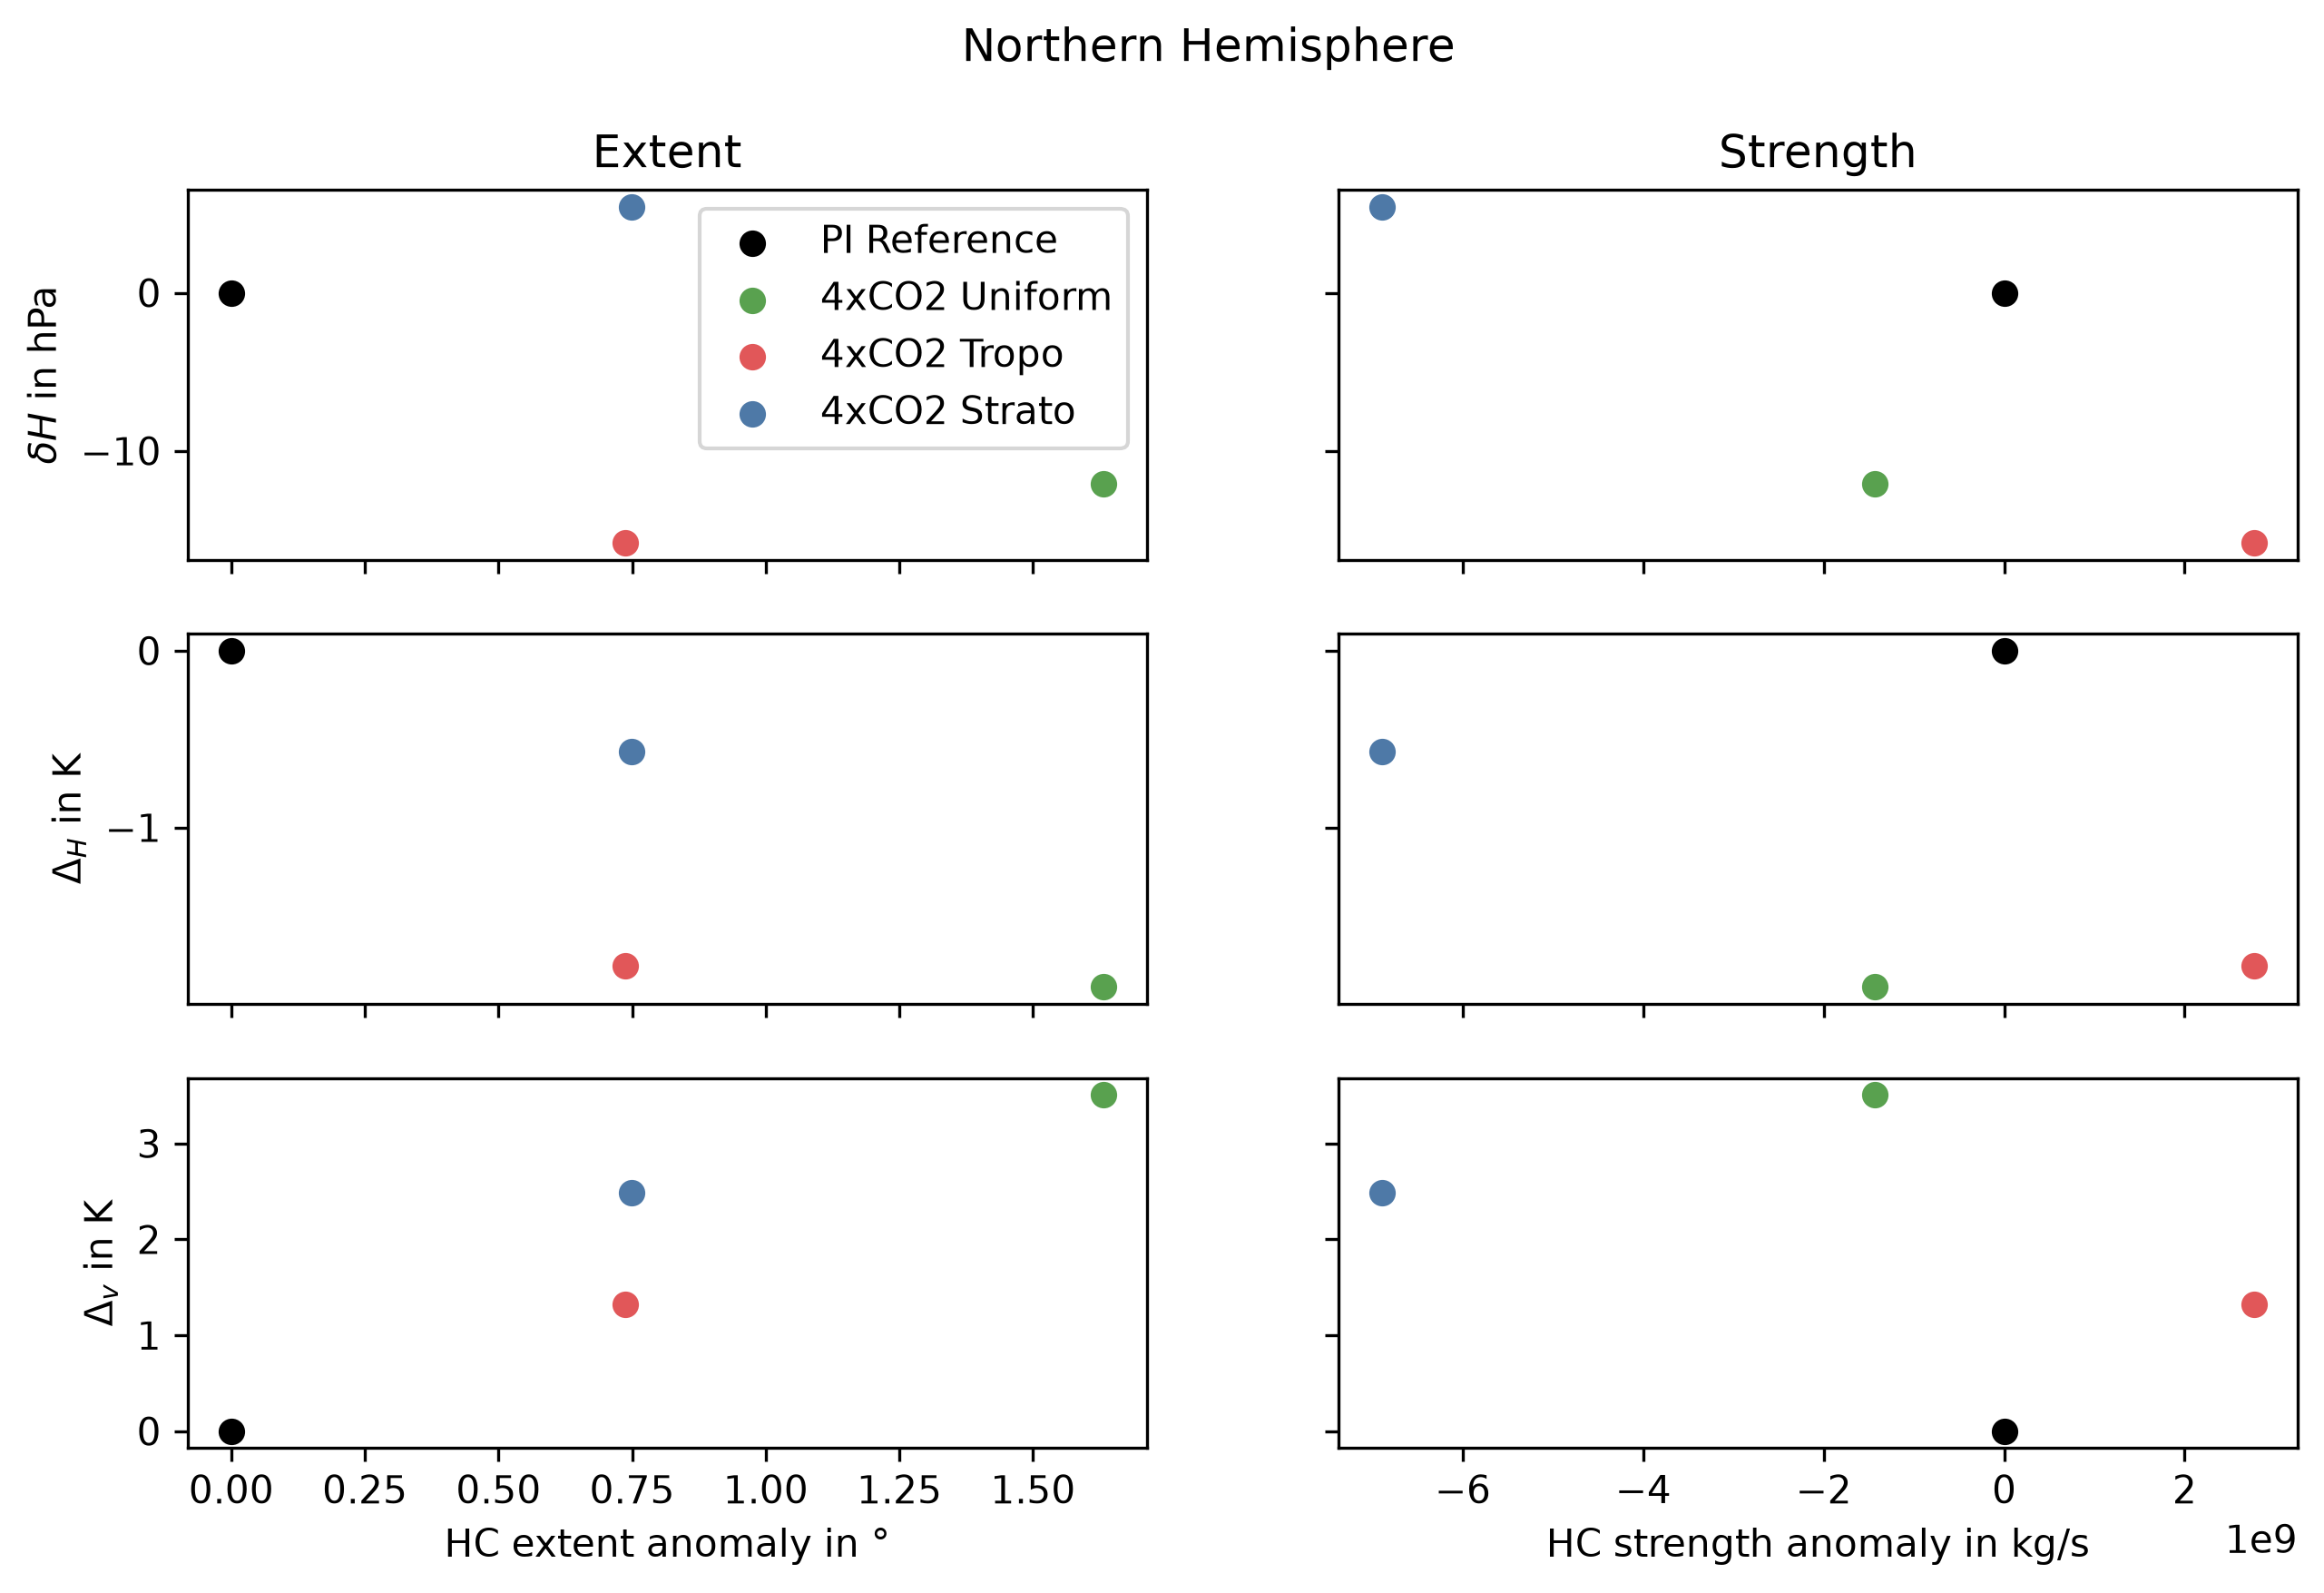
\includegraphics[width=\textwidth]{../../figures/H&H/parameters_NH.png}
    \end{figure}
\end{frame}
\begin{frame}
    \frametitle{}
    \begin{figure}
        \centering
        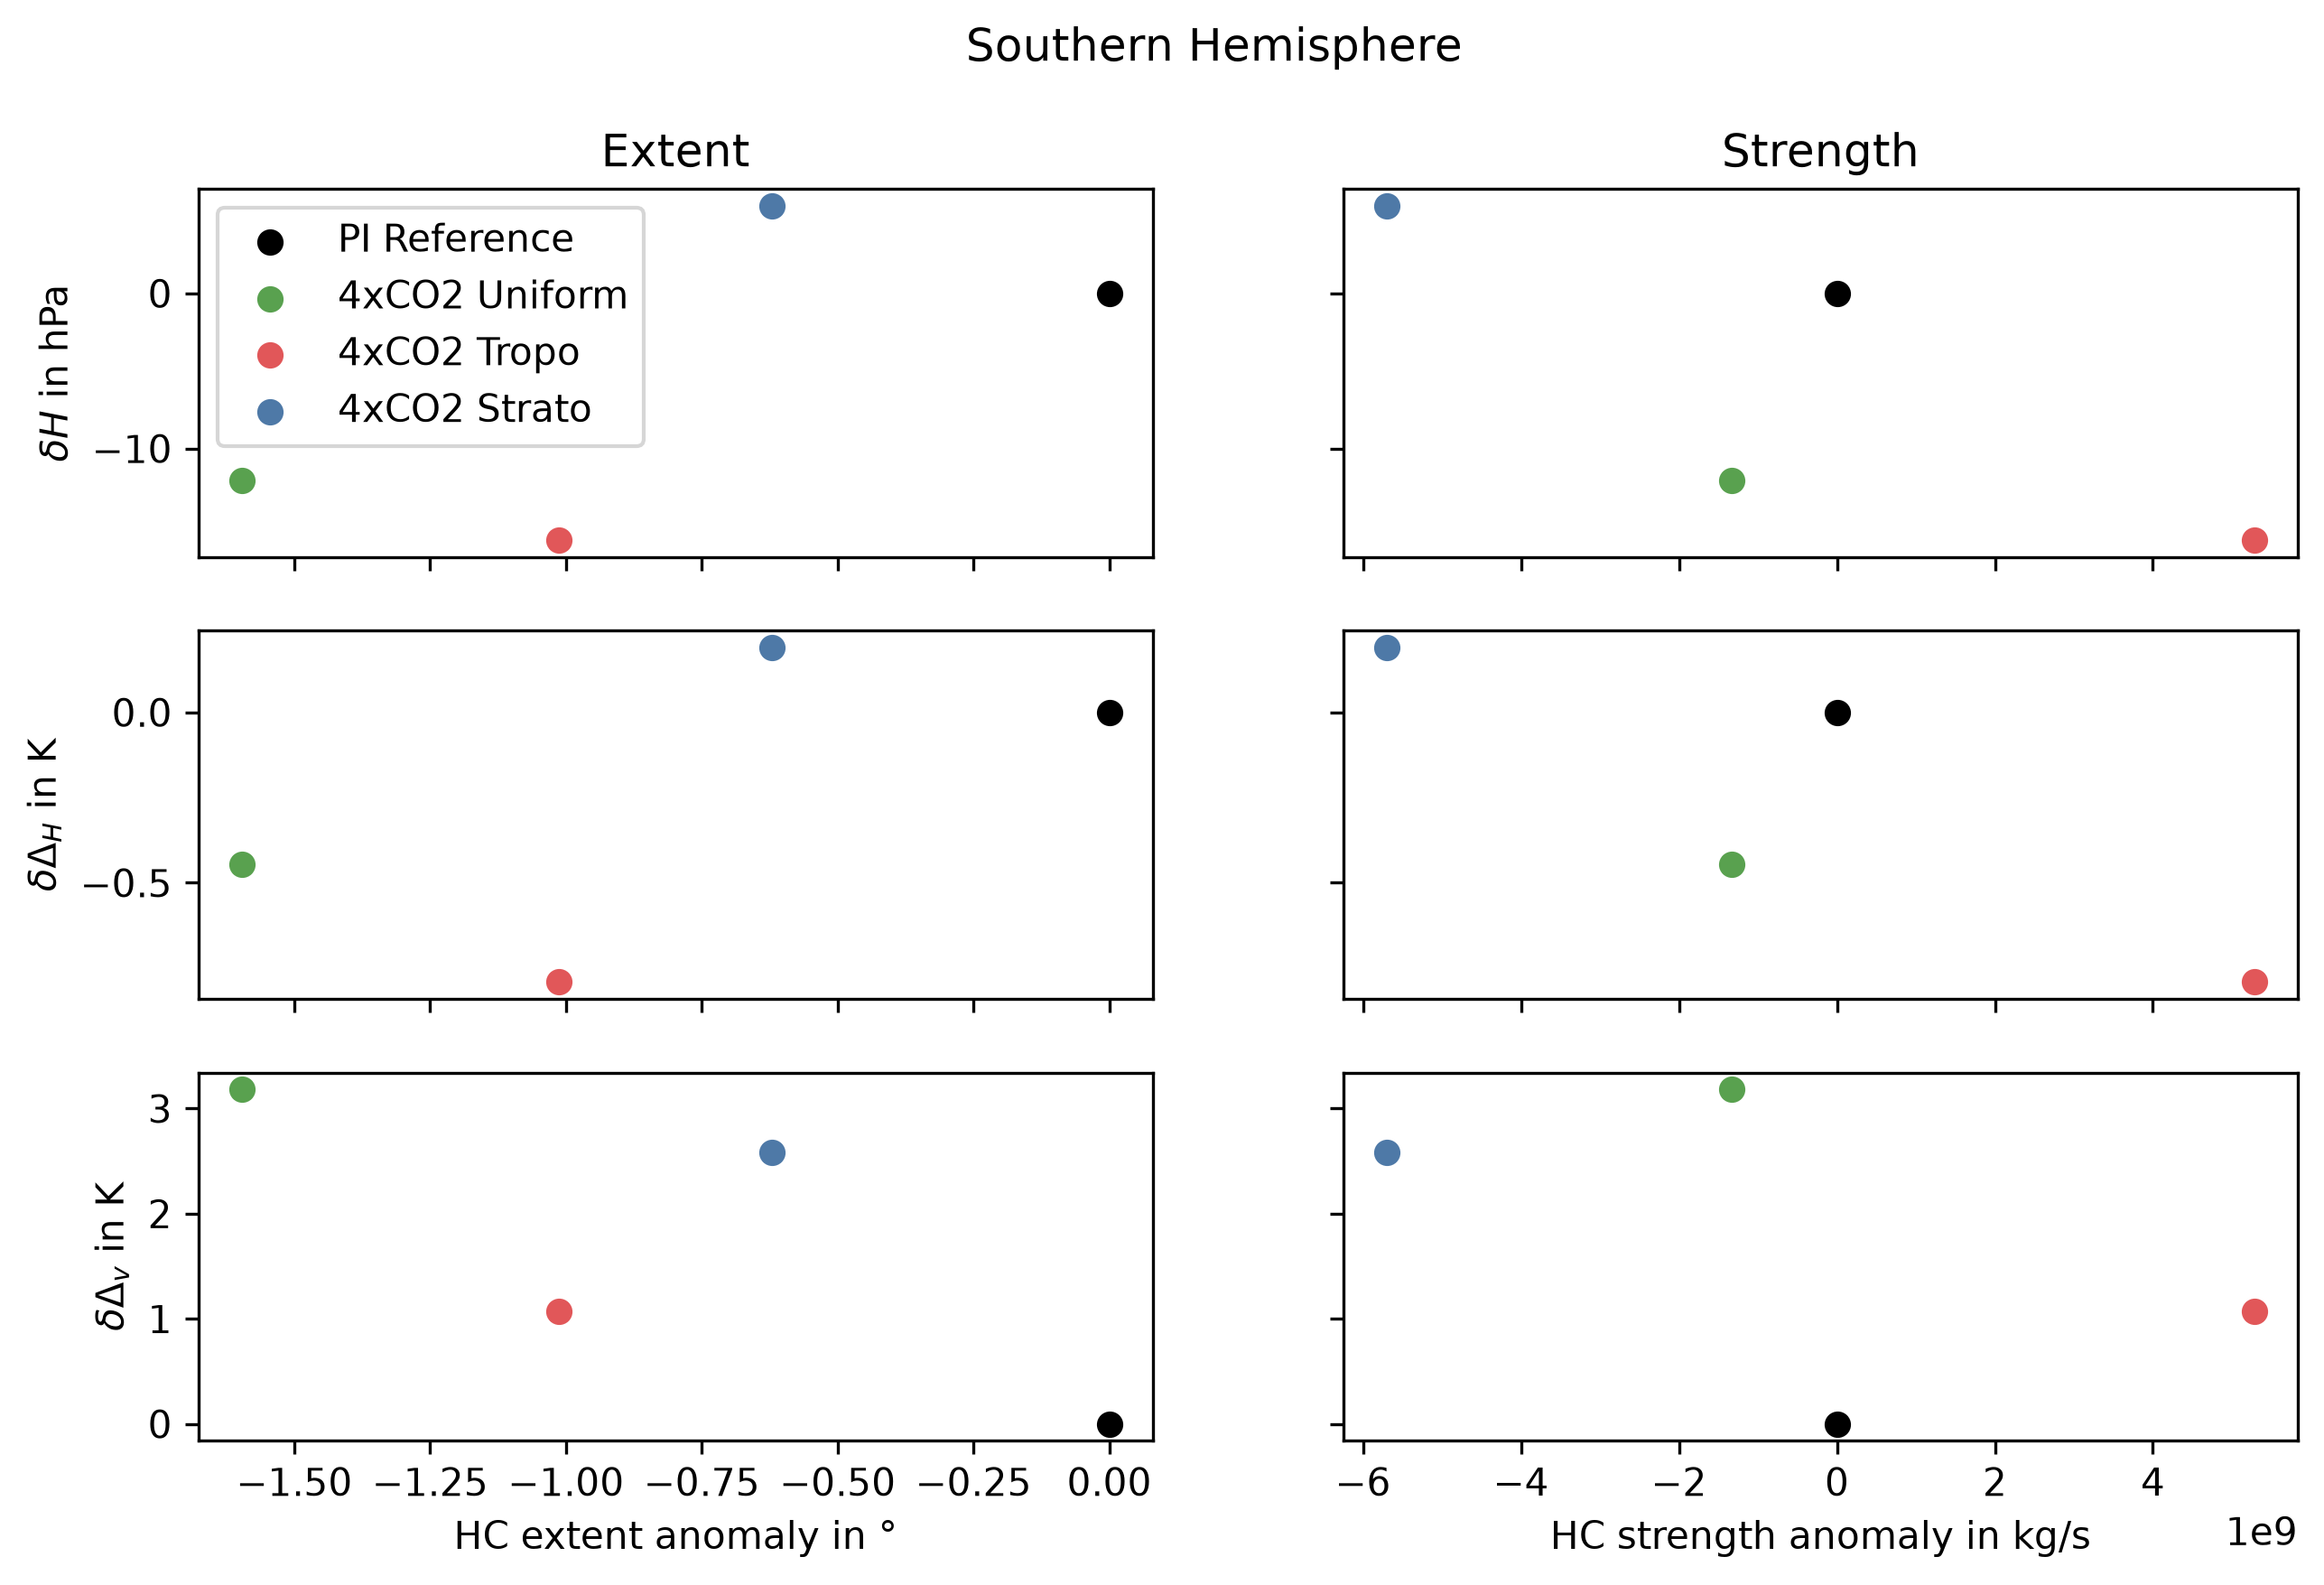
\includegraphics[width=\textwidth]{../../figures/H&H/parameters_SH.png}
    \end{figure}
\end{frame}

\begin{frame}
    \frametitle{}
    \begin{figure}
        \centering
        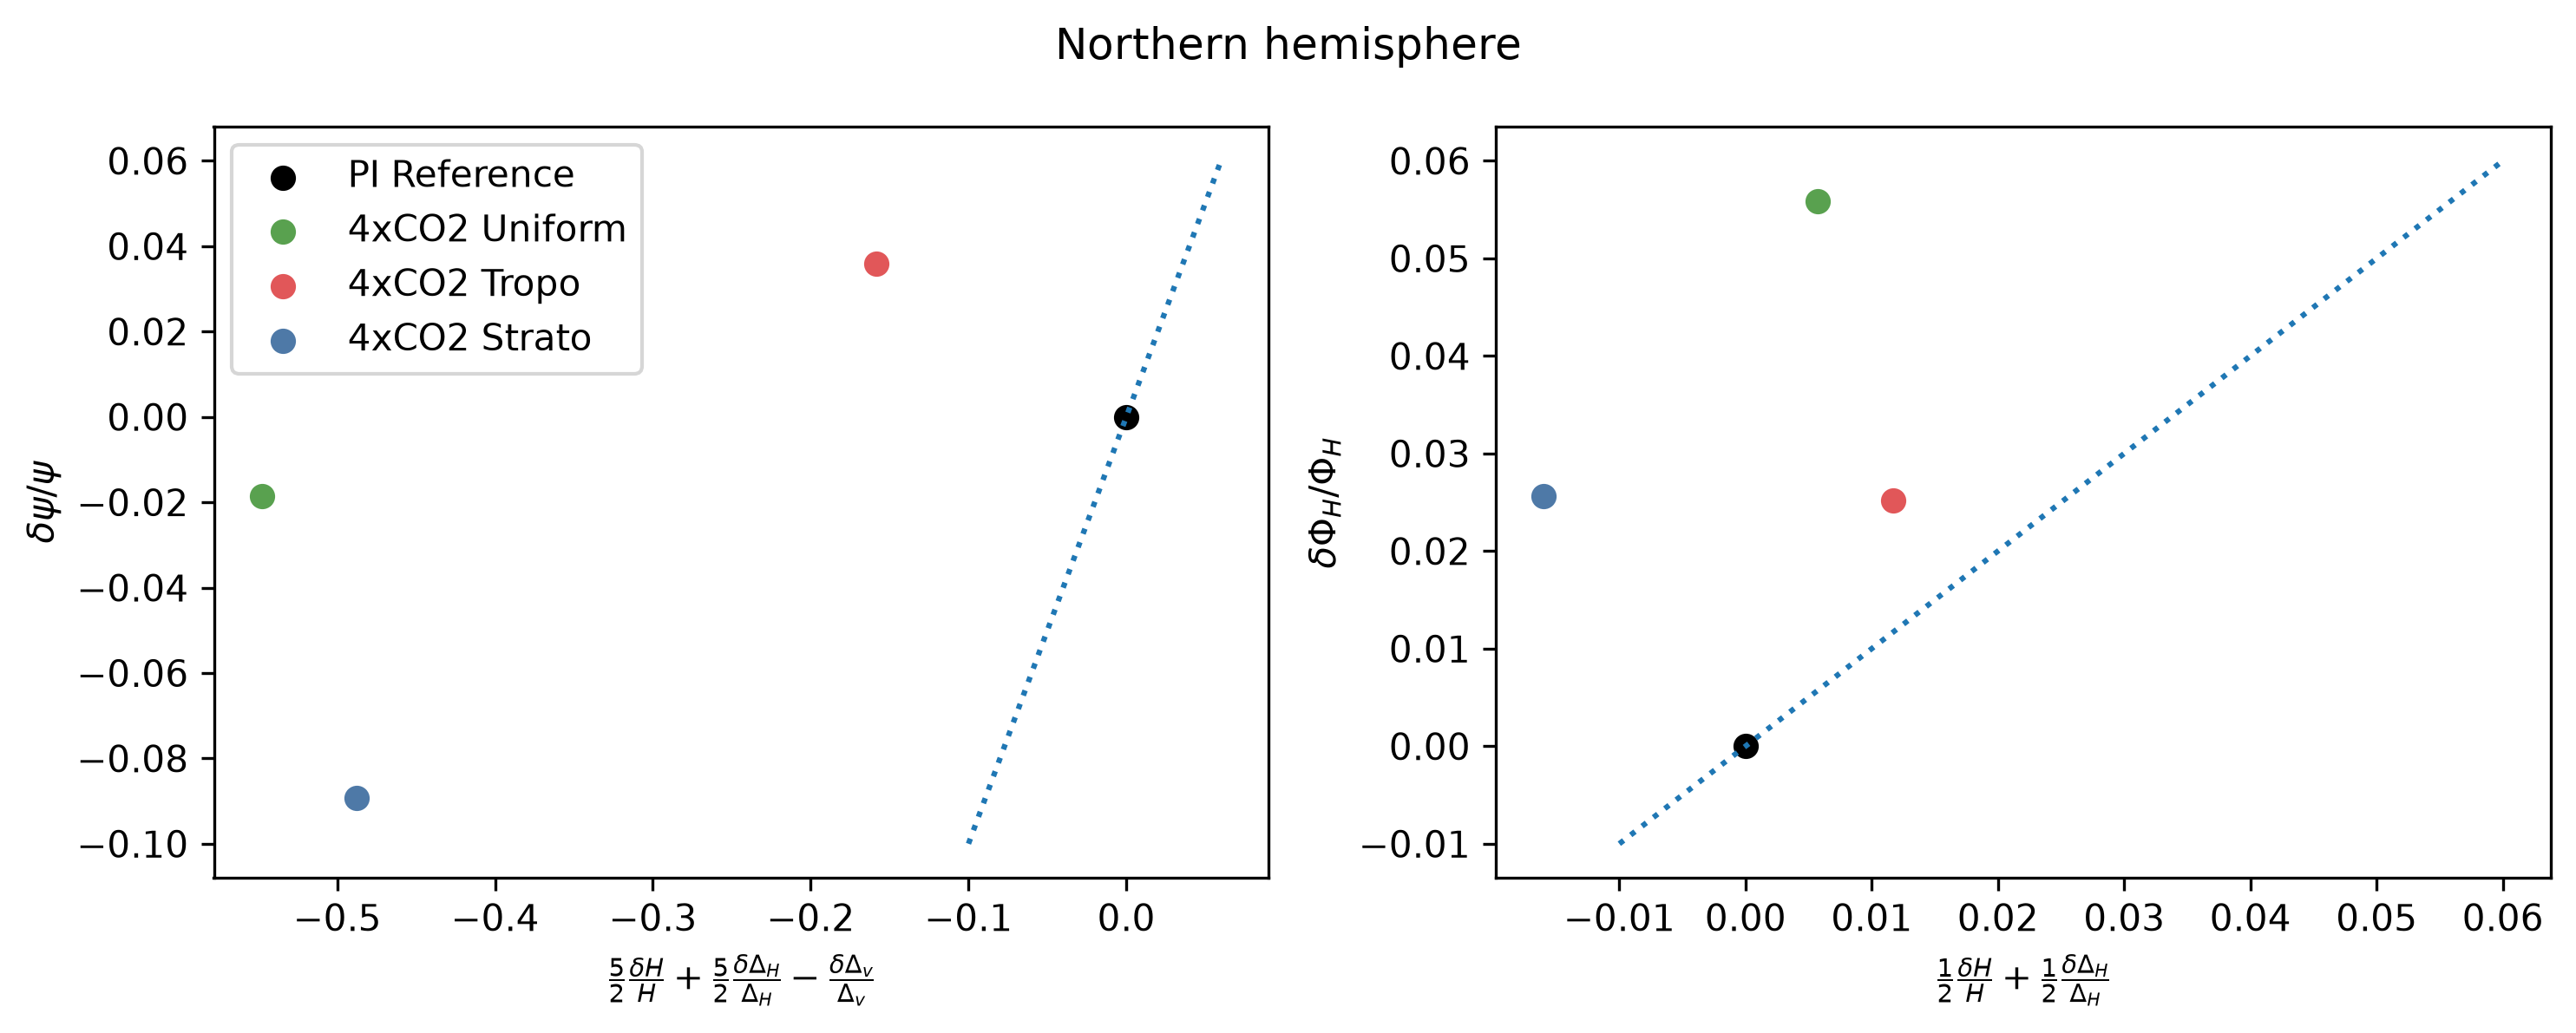
\includegraphics[width=\textwidth]{../../figures/H&H/scatter_NH.png}
    \end{figure}
\end{frame}
\begin{frame}
    \frametitle{}
    \begin{figure}
        \centering
        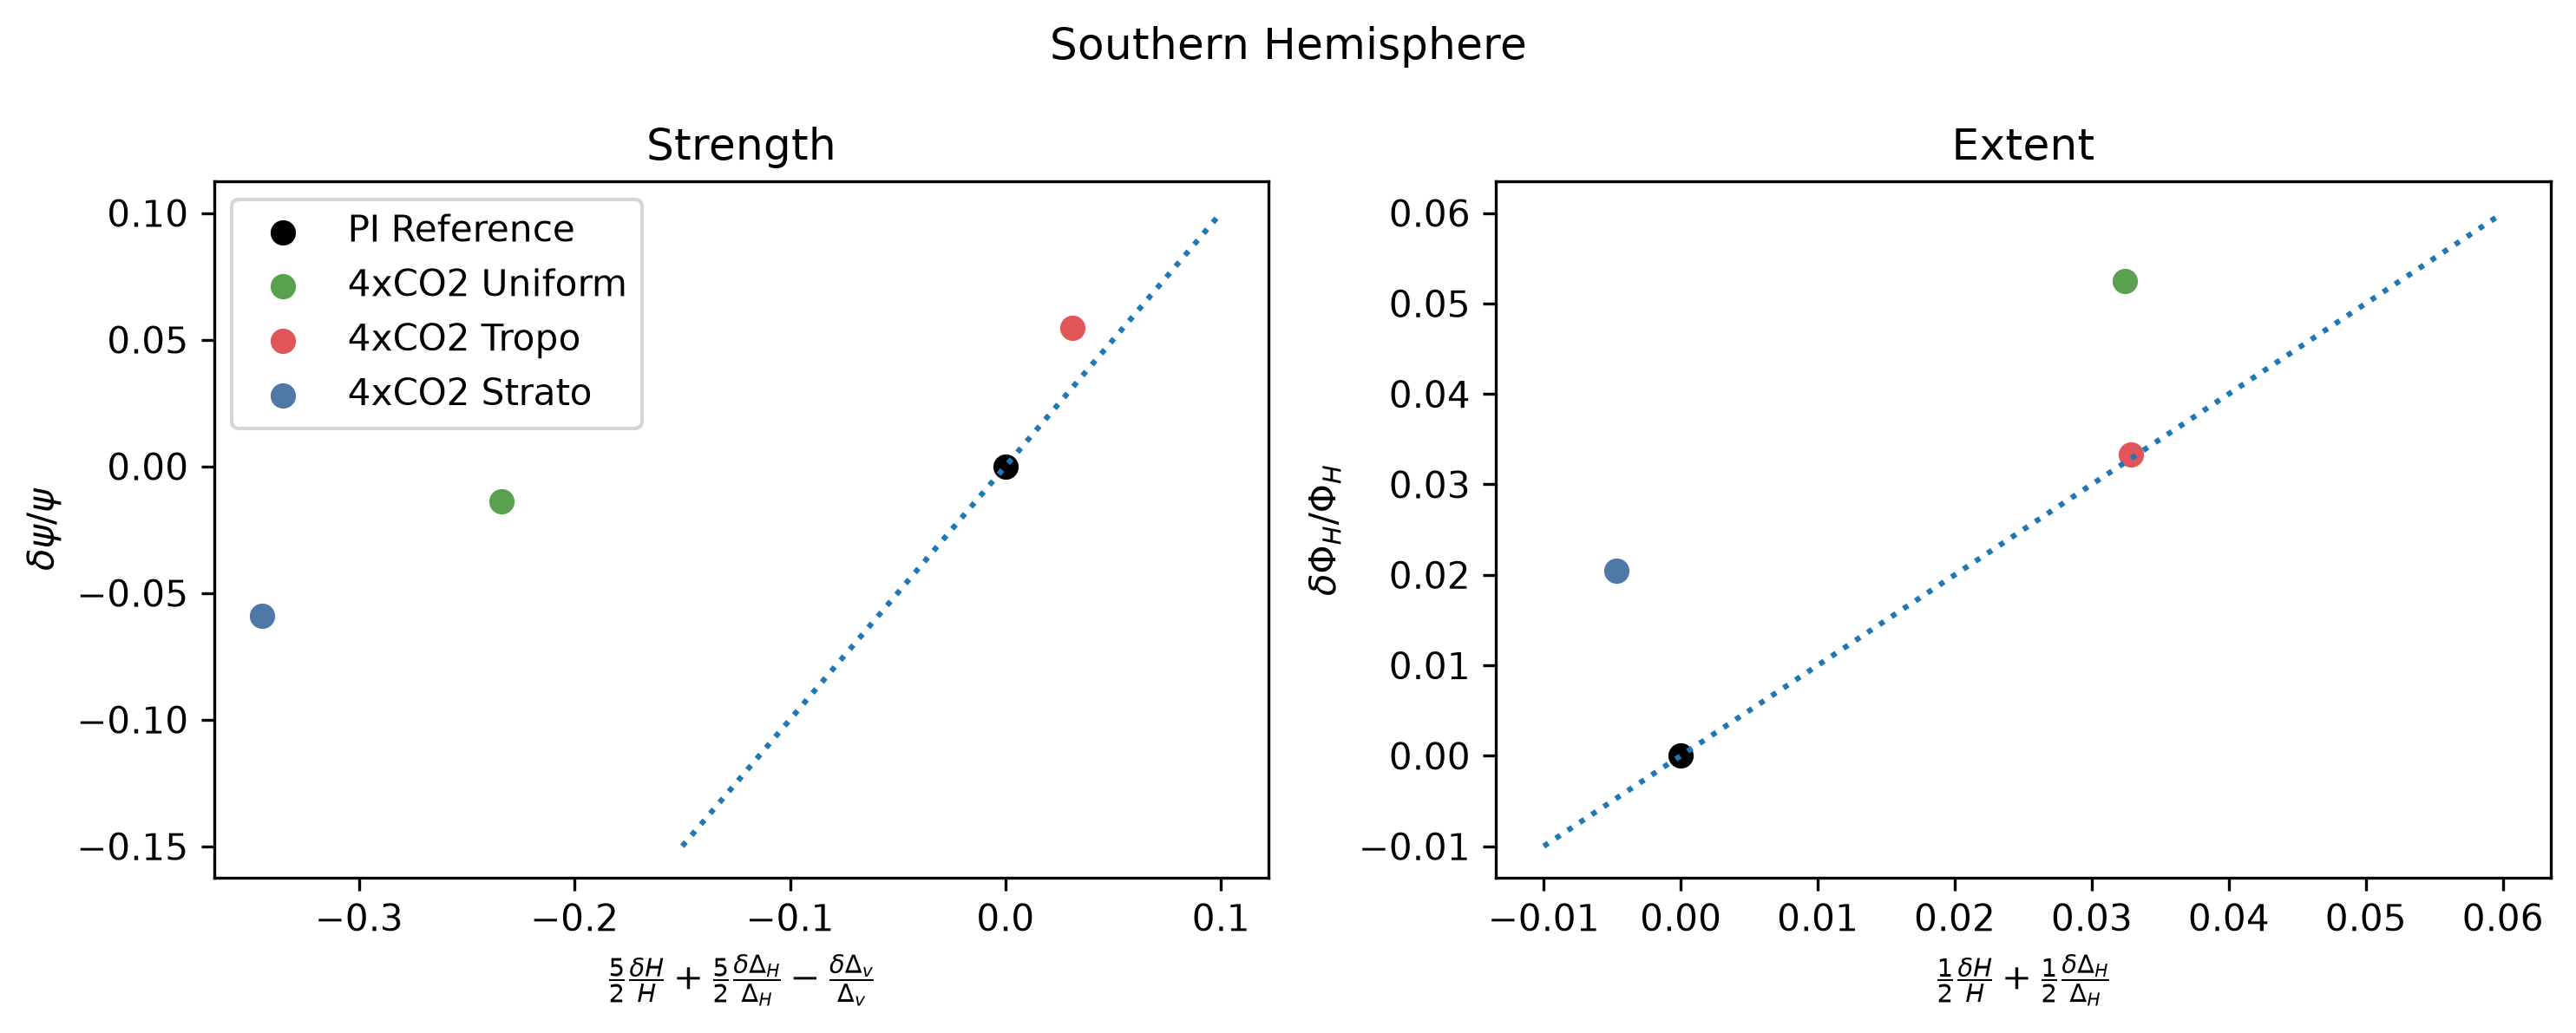
\includegraphics[width=\textwidth]{../../figures/H&H/scatter_SH.png}
    \end{figure}
\end{frame}


\begin{frame}
    \frametitle{Eddy anomalies}
    \begin{figure}
        \centering
        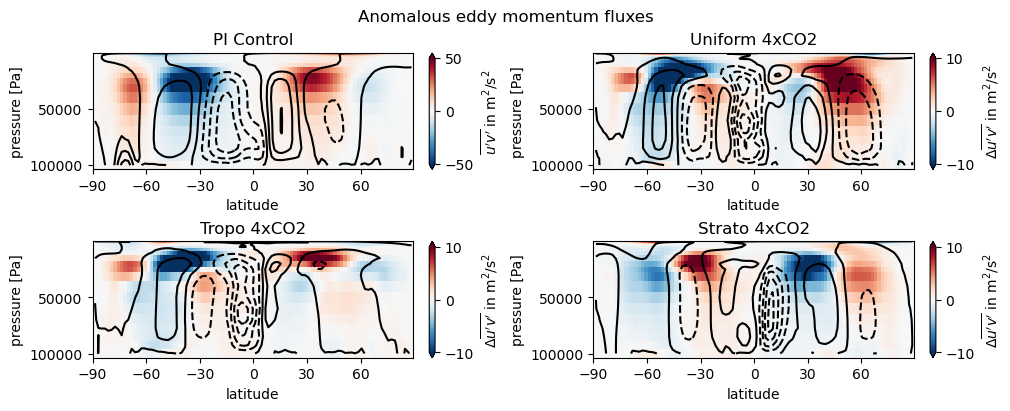
\includegraphics[width=\textwidth]{../../figures/eddy_flux/anomalous_uv.png}
    \end{figure}
\end{frame}

\begin{frame}
    \frametitle{}
    \begin{figure}
        \centering
        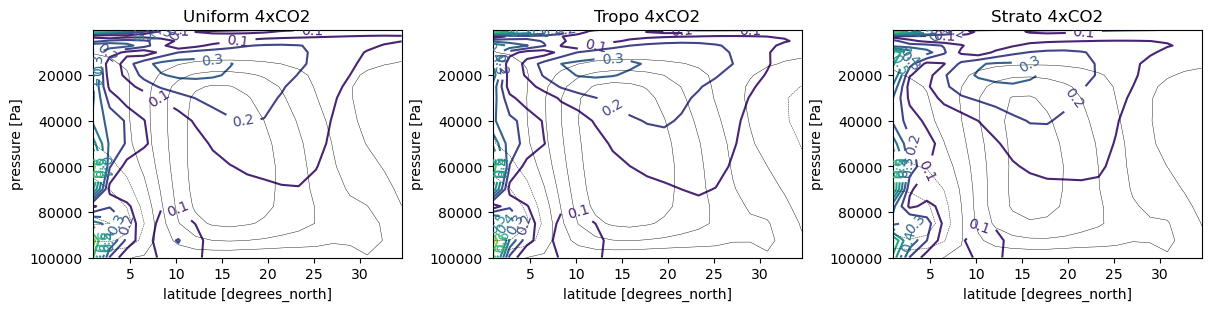
\includegraphics[width=\textwidth]{../../figures/eddy_flux/local_Ro.png}
    \end{figure}
\end{frame}
\begin{frame}
    \frametitle{HC strength versus eddy driven HC strength}
    \begin{figure}
        \centering
        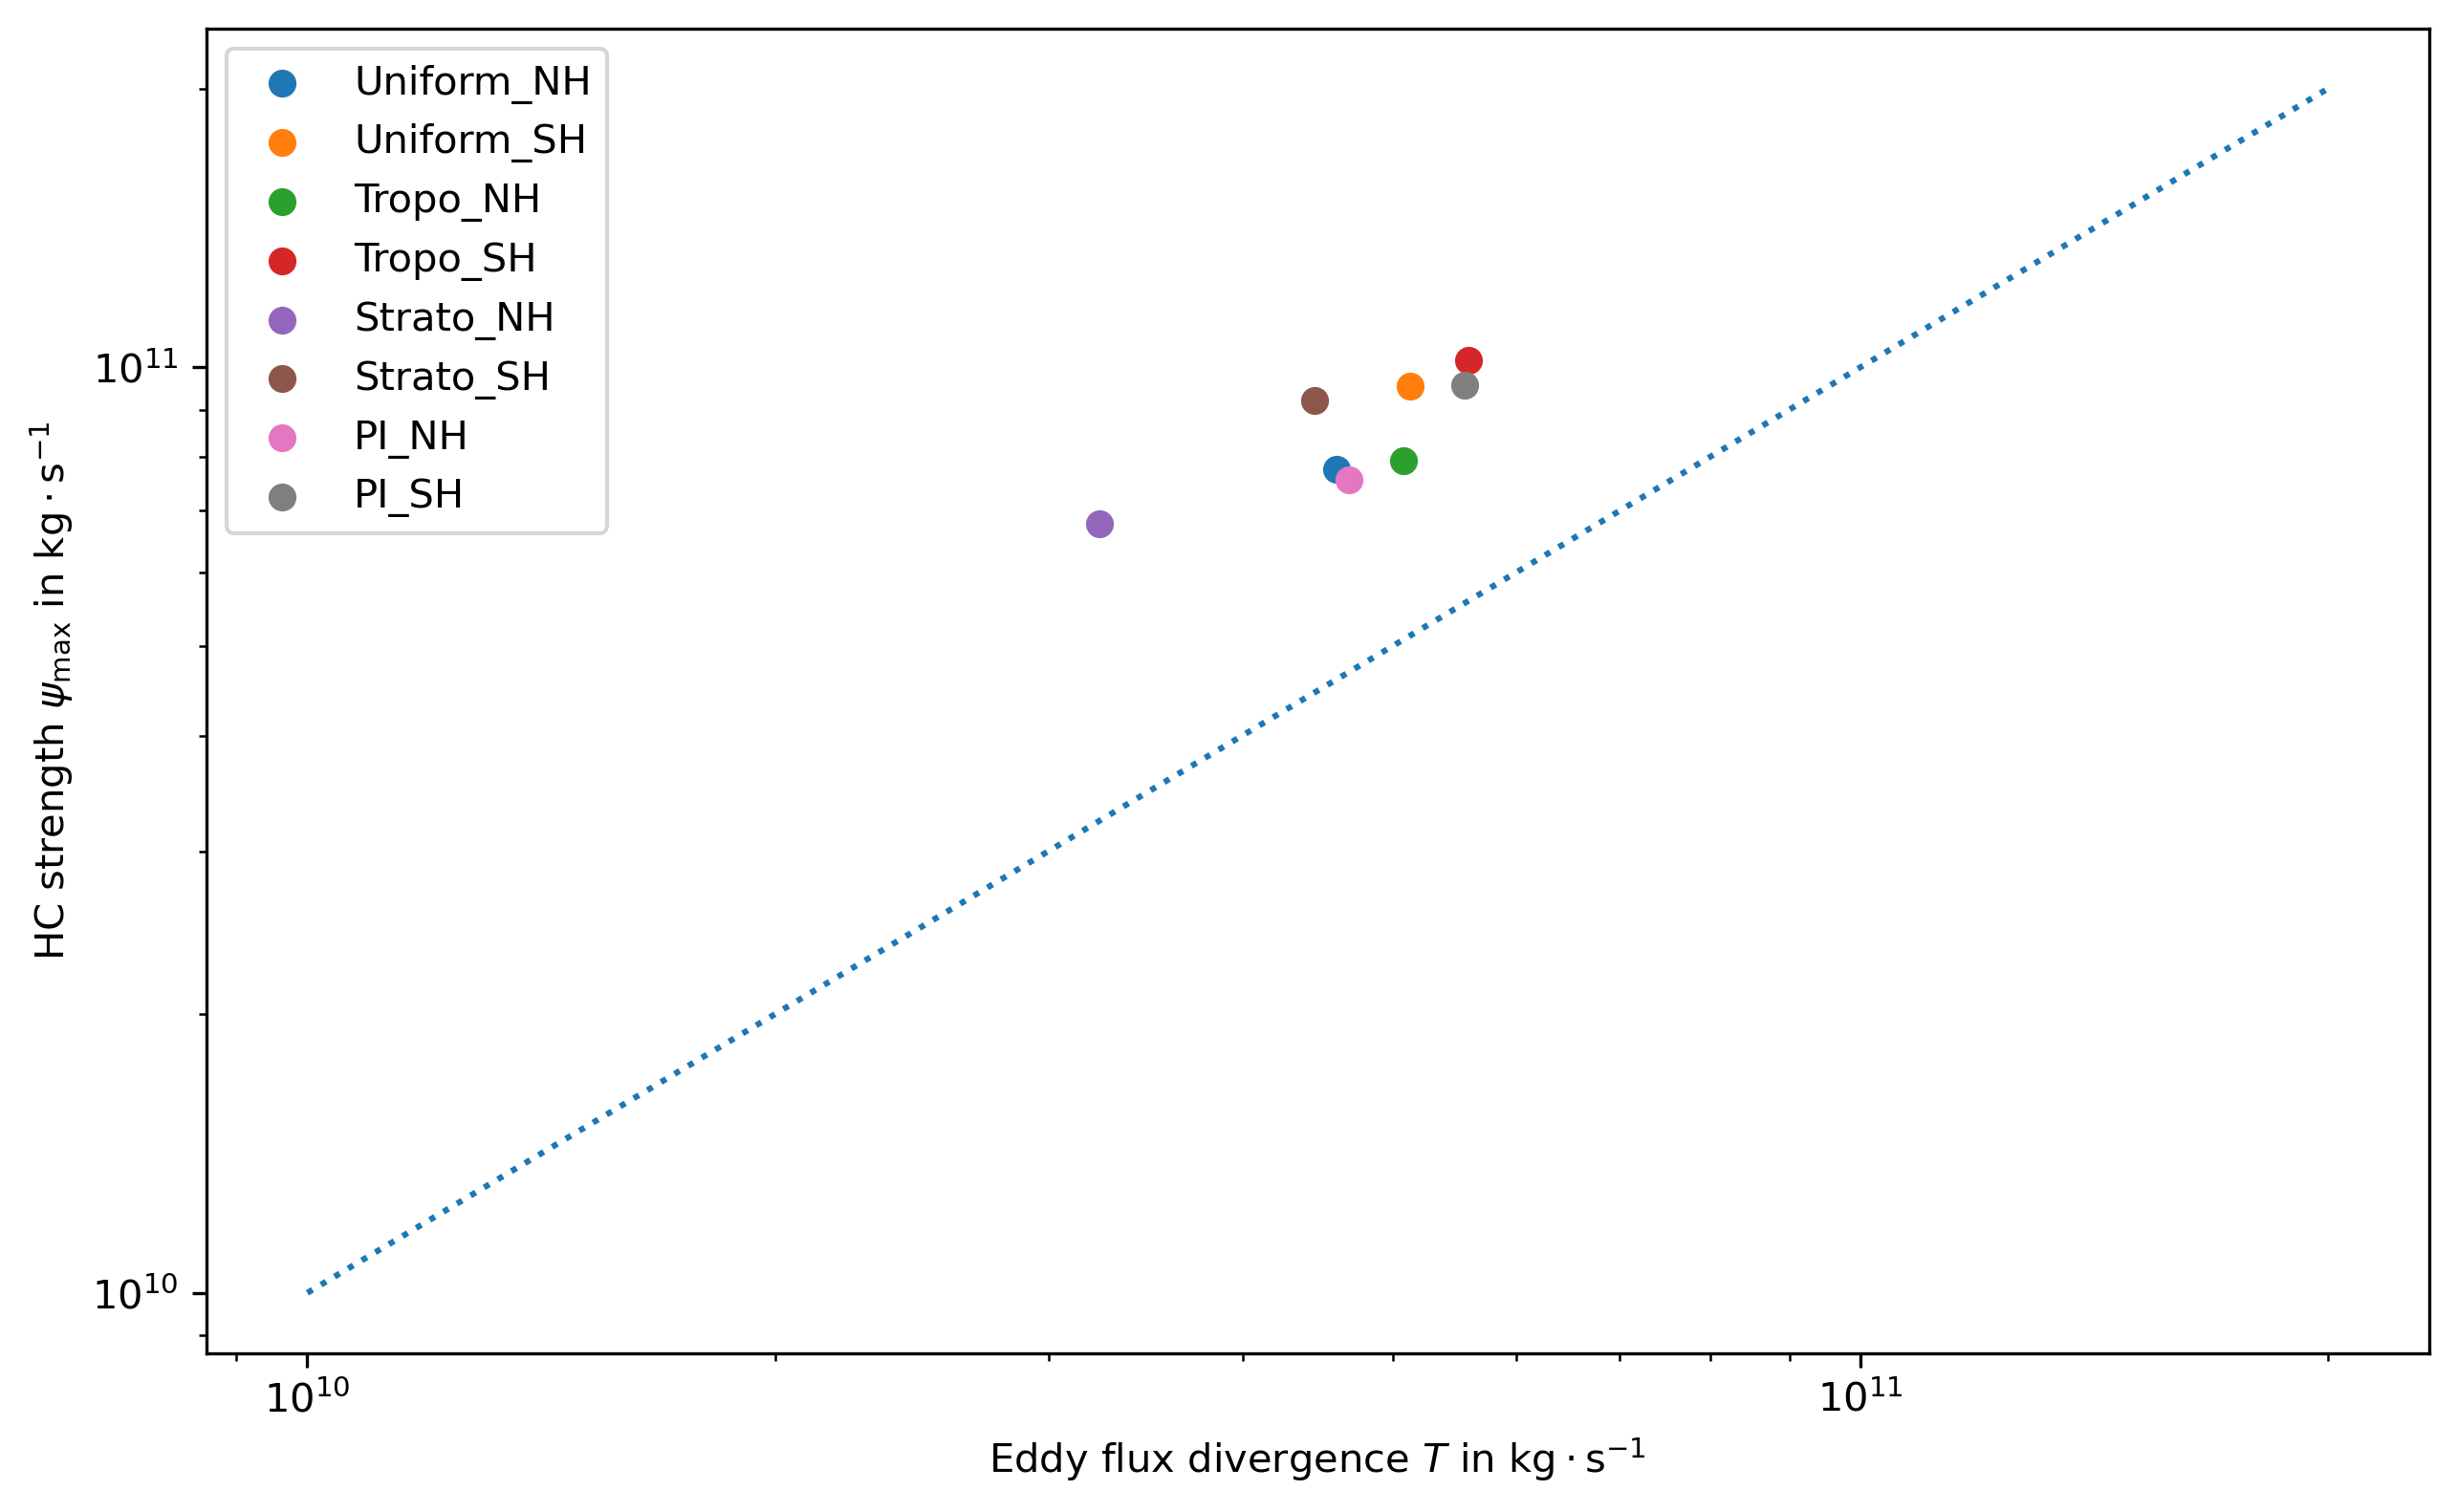
\includegraphics[width=\textwidth]{../../figures/eddy_flux/eddy_flux_vs_strength.png}
    \end{figure}
\end{frame}

\begin{frame}
    \frametitle{Ferrel cell strength versus eddy driven Ferrel cell strength}
    \begin{figure}
        \centering
        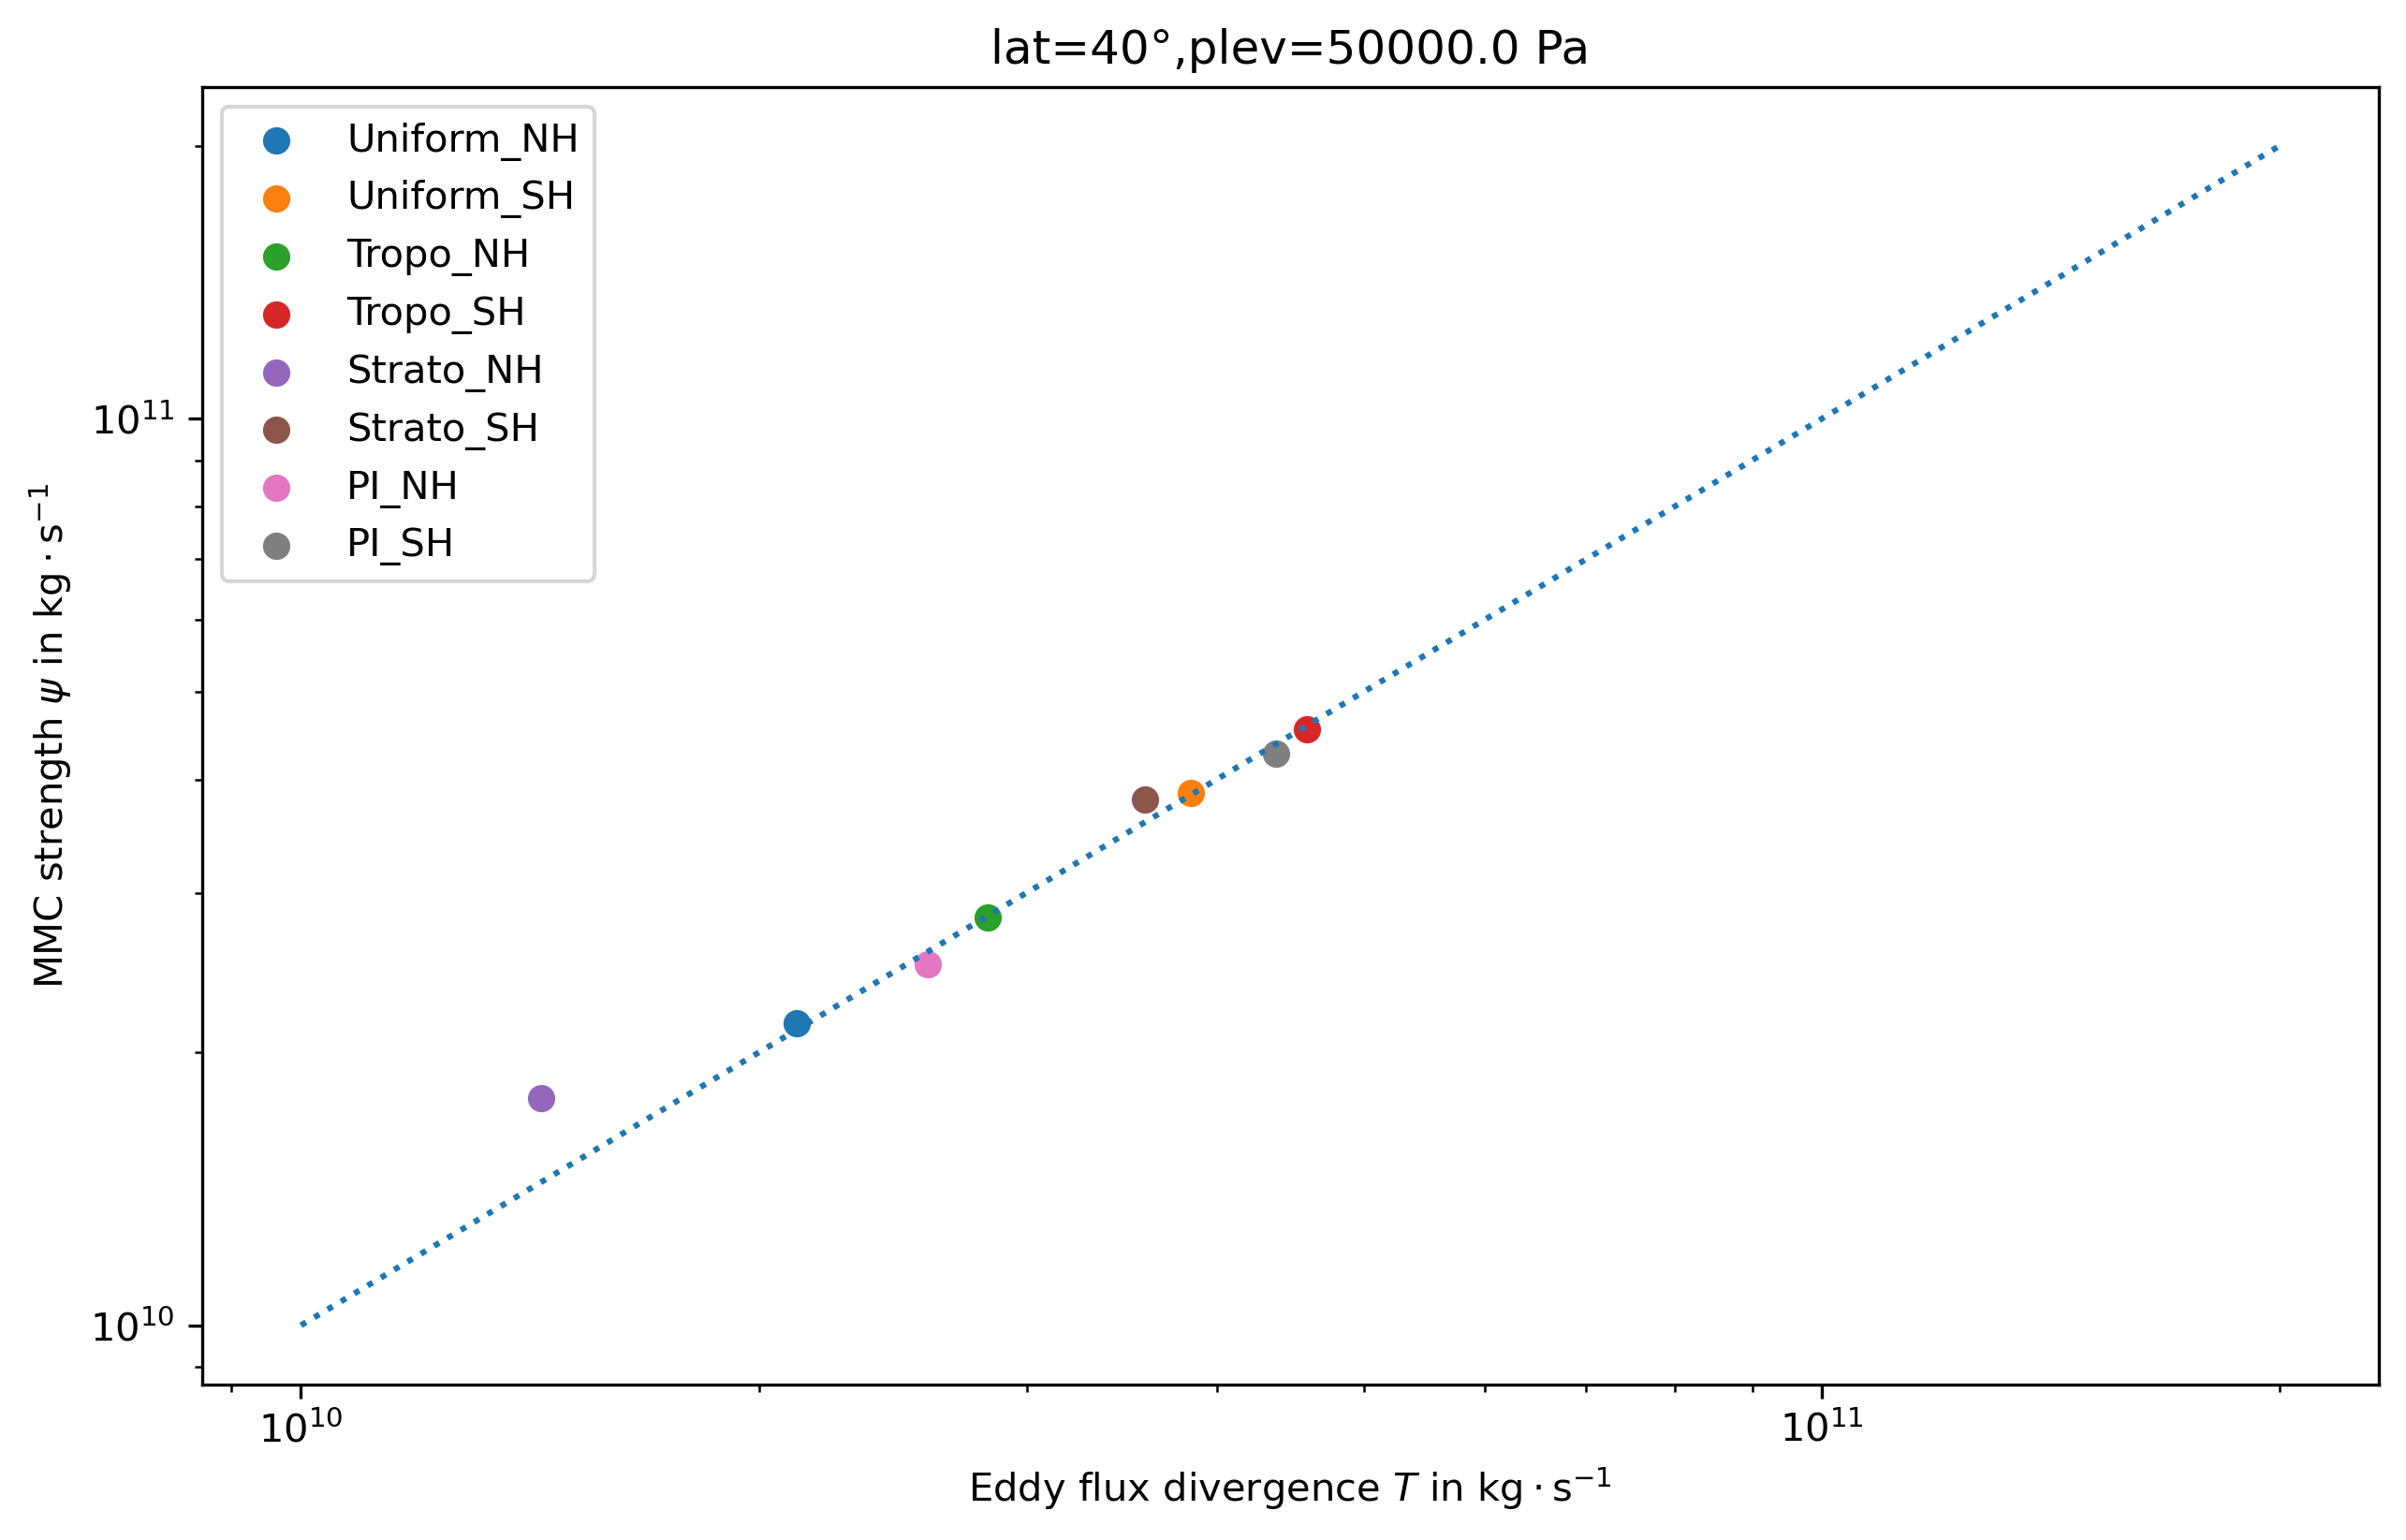
\includegraphics[width=\textwidth]{../../figures/eddy_flux/ferrell_cell_eddy_flux_vs_strength.png}
    \end{figure}
\end{frame}

\begin{frame}
    \frametitle{Seasonality}
    \begin{figure}
        \centering
        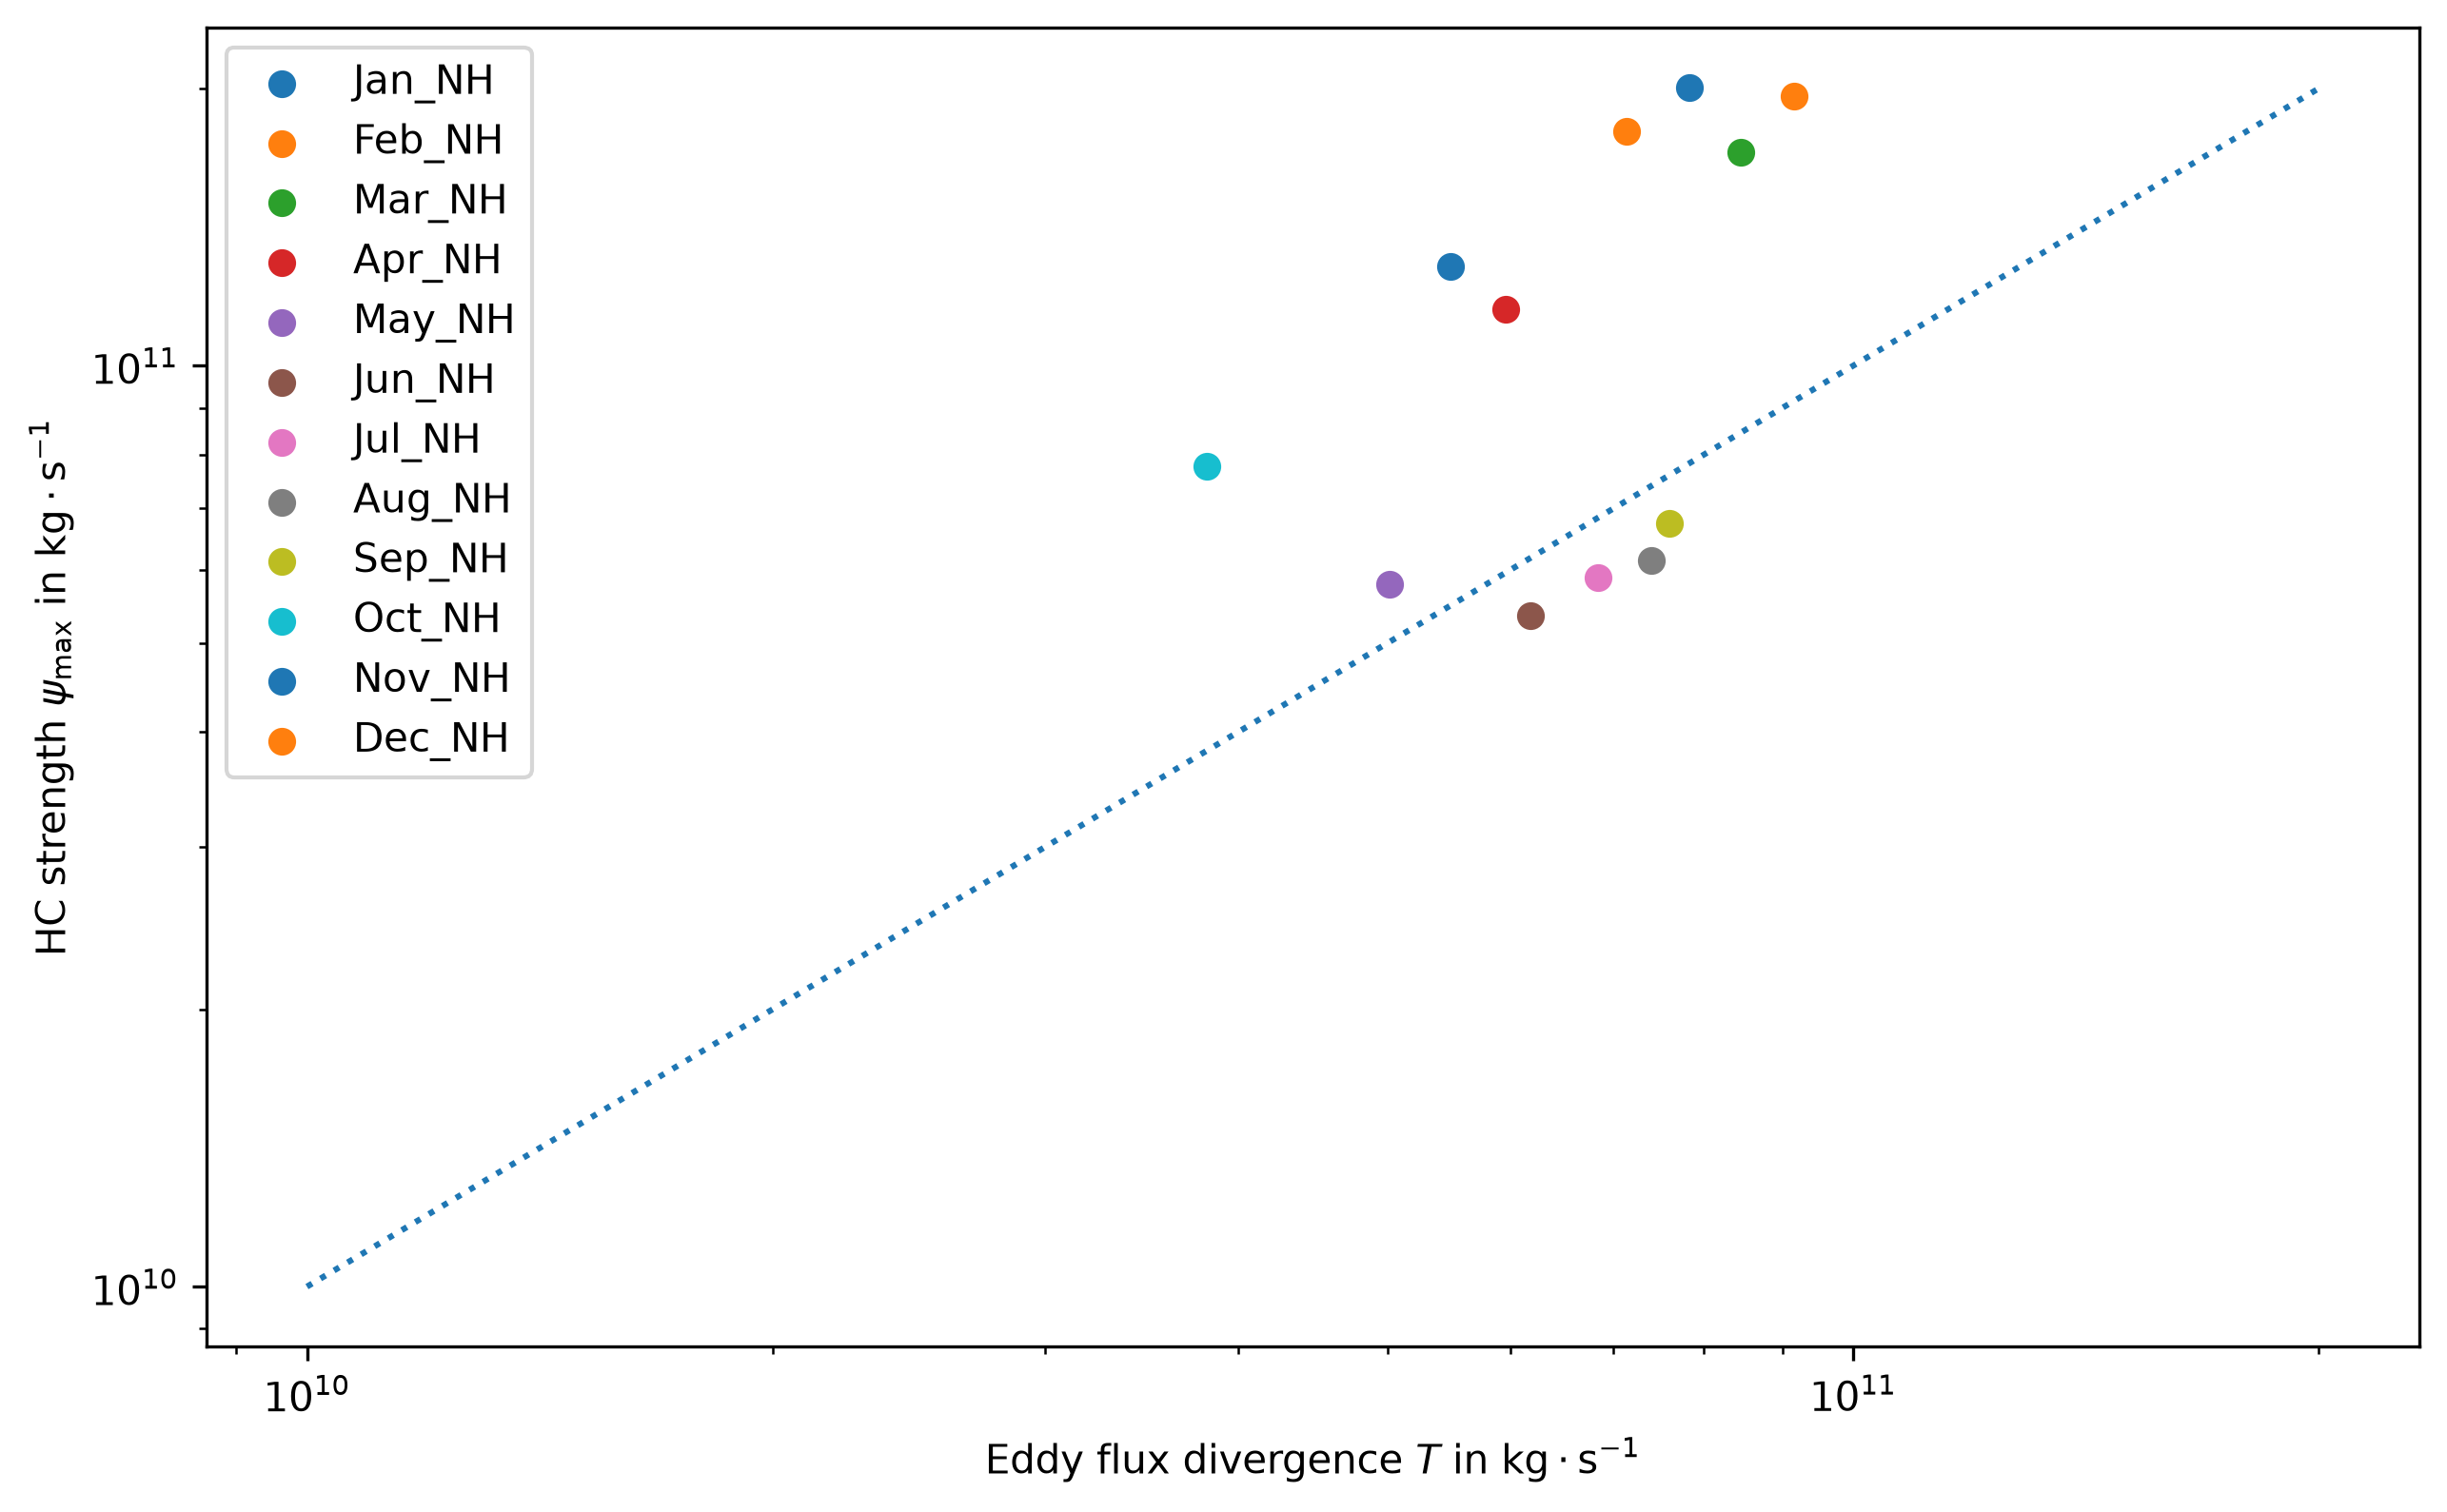
\includegraphics[width=\textwidth]{../../figures/eddy_flux/eddies_strength_seasonal.png}
    \end{figure}
\end{frame}

\begin{frame}
    \frametitle{SW LW clear sky}
    \begin{figure}
        \centering
        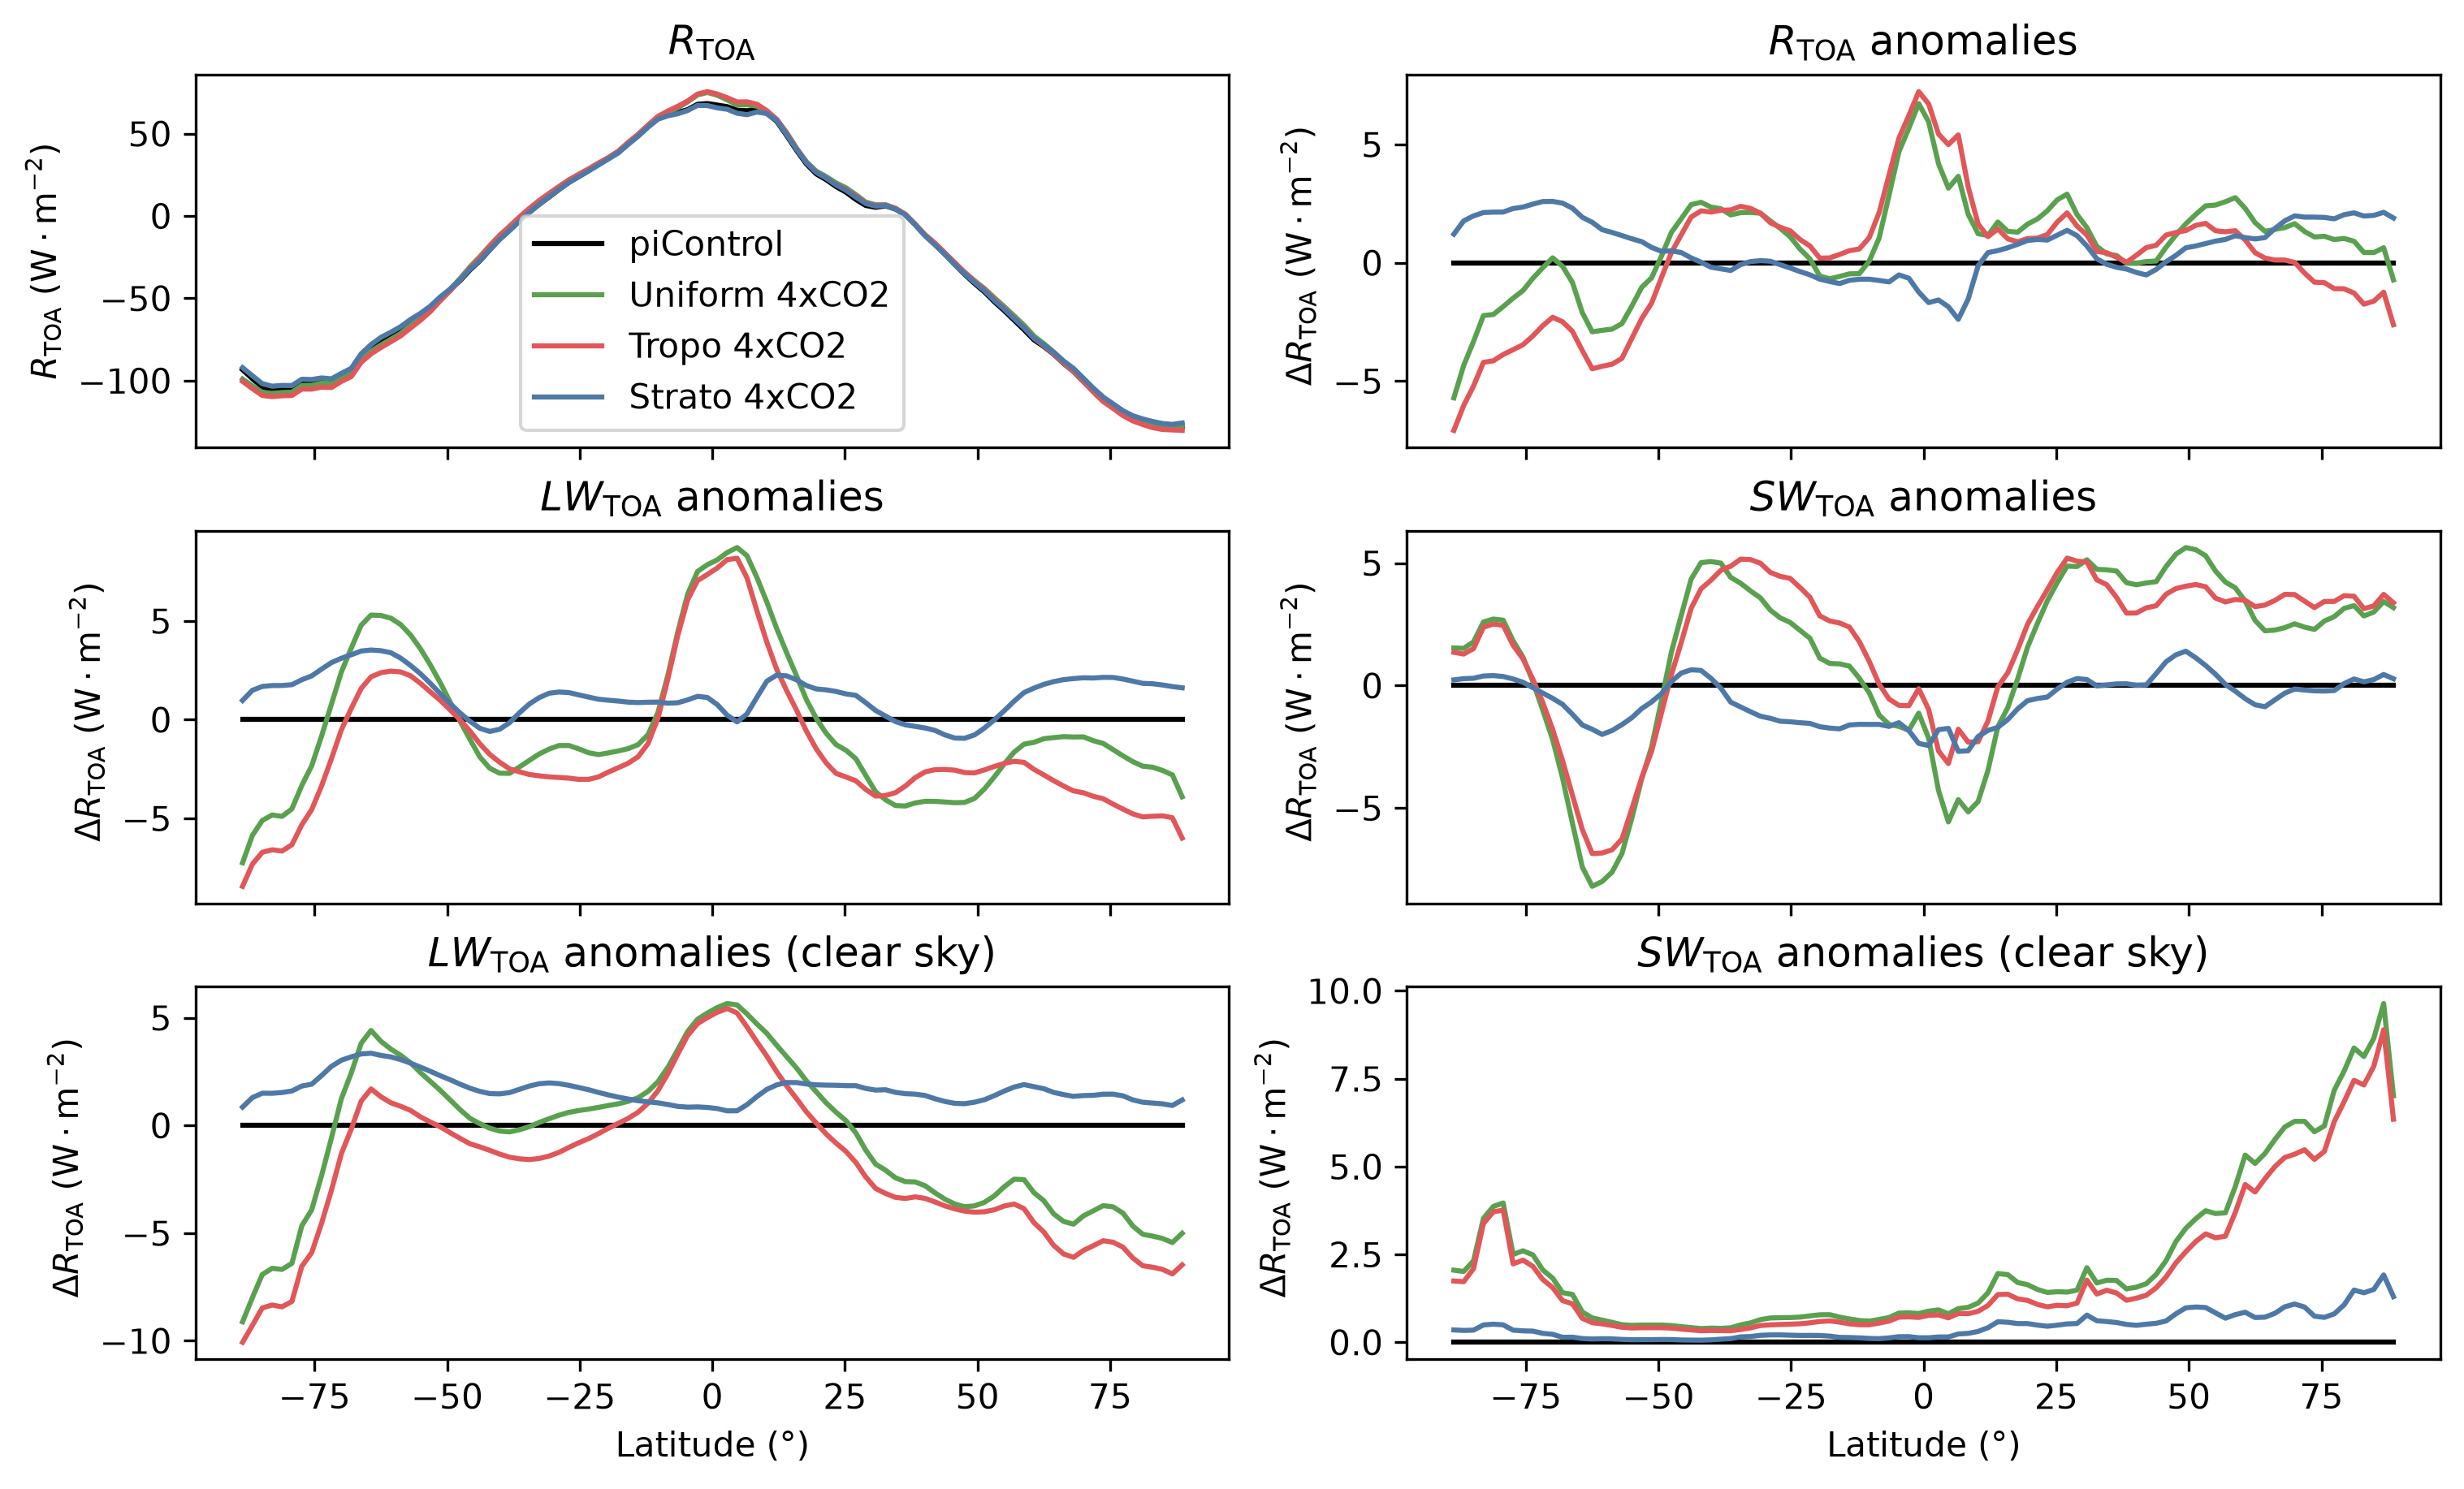
\includegraphics[width=\textwidth]{../../figures/energetic_framework/TOA_fluxes.png}
    \end{figure}
\end{frame}

\begin{frame}
    \frametitle{Sea ice (ocean transport)}
    \begin{figure}
        \centering
        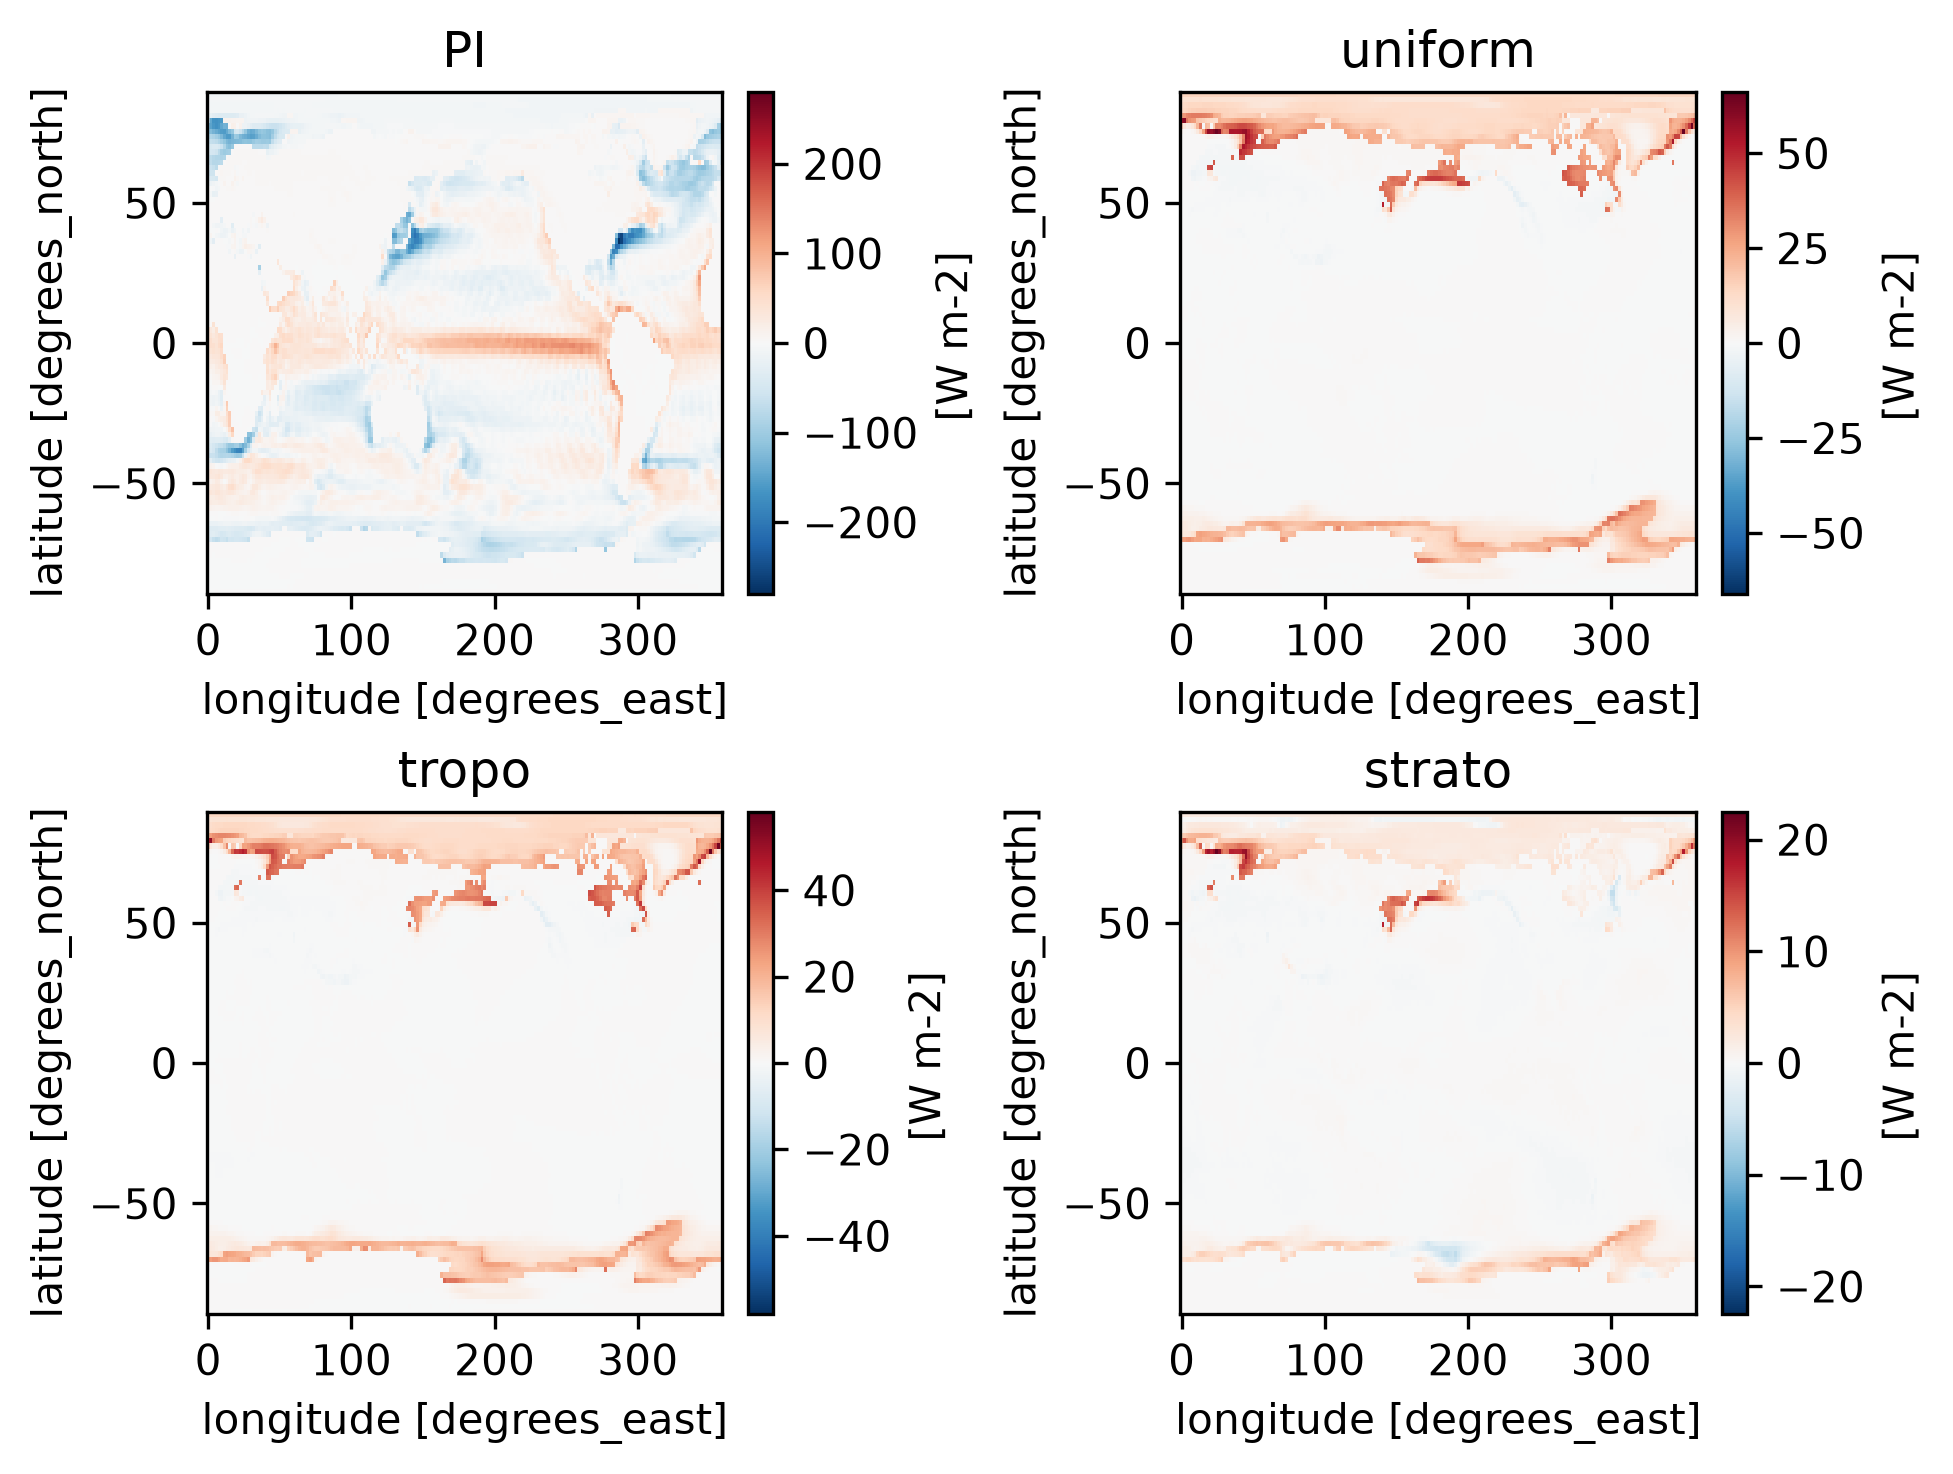
\includegraphics[width=0.8\textwidth]{../../figures/energetic_framework/R_surf_anomalies_spatially_sea_ice.png}
    \end{figure}
\end{frame}

\backupend
\end{document}
